\documentclass[12pt, landscape]{article}
\usepackage[scaled=0.92]{helvet}
\usepackage{multicol}
\usepackage{calc}
\usepackage{ifthen}
\usepackage[landscape]{geometry}
%\usepackage{hyperref}

\usepackage{newtxtext} 

%for strikeout
\usepackage{ulem}

%For editing parbox
\usepackage[table]{xcolor}
%For editing itemise margins, reduce iterm separaion and list separation
\usepackage{enumitem}
% For math
\usepackage{amsmath,amsthm,amsfonts,amssymb}

%For pictures / figures
\usepackage{color,graphicx,overpic}
\graphicspath{ {./../images/} }

%\usepackage{newtxtext} 
%\usepackage{amssymb}
%\usepackage[table]{xcolor}
%\usepackage{vwcol}
%\usepackage{tikz}
%\usepackage{wrapfig}
%\usepackage{makecell}


% For Code Blocks
\usepackage{xcolor}
\usepackage{listings}

\lstdefinestyle{mystyle}{
	backgroundcolor=\color{gray!25!white},
	basicstyle=\scriptsize,
	numbers=none,    %or = none or left
	showstringspaces=false,
	breaklines=true,
	breakatwhitespace=false,                  
	captionpos=b,                    
	keepspaces=true,                                 
	numbersep=5pt,                  
	showspaces=false,                
	showtabs=false,                  
	tabsize=2,
 }
%Helpful:
%[linewidth = 1.0 \linewidth]
%\lstinline{}
% use \code{} for \lstinline with colorbox.
\newcommand{\code}[1]{\colorbox{gray!25!}{\lstinline|#1|}}
\lstset{style=mystyle}

% Template: Cheatsheet with code enabled

%--------------------------- PACKAGES ABOVE --------------------------------------------------------------

\pdfinfo{
  /Title (Documentname.pdf)
  /Creator (Ger Teck)
  /Author (Ger Teck)
  /Subject ()
  /Keywords (tex)}

%% Margins for PAPER

% This sets page margins to .5 inch if using letter paper, and to 1cm
% if using A4 paper. (This probably isn't strictly necessary.)
% If using another size paper, use default 1cm margins.
\ifthenelse{\lengthtest { \paperwidth = 11in}}
	{ \geometry{top=.5in,left=.5in,right=.5in,bottom=.5in} }
	{\ifthenelse{ \lengthtest{ \paperwidth = 297mm}}
		{\geometry{top=1cm,left=1cm,right=1cm,bottom=1cm} }
		{\geometry{top=1cm,left=1cm,right=1cm,bottom=1cm} }
	}

% Turn off header and footer
\pagestyle{empty}

% for tight centres (less spacing)
\newenvironment{tightcenter}{%
  \setlength\topsep{0.5pt}
  \setlength\parskip{0.5pt}
  \begin{center}
}{%
  \end{center}
}

% Redefine section commands to use less space
\makeatletter
\renewcommand{\section}{\@startsection{section}{1}{0mm}%
                                {-1ex plus -.5ex minus -.2ex}%
                                {0.5ex plus .2ex}%x
                                {\normalfont\large\bfseries}}
\renewcommand{\subsection}{\@startsection{subsection}{2}{0.1mm}%
                                {-1explus -.5ex minus -.2ex}%
                                {0.5ex plus .2ex}%
                                {\normalfont\normalsize\bfseries}}
\renewcommand{\subsubsection}{\@startsection{subsubsection}{3}{0.1mm}%
                                {-1ex plus -.5ex minus -.2ex}%
                                {1ex plus .2ex}%
                                {\normalfont\small\bfseries}}
% change font
%\renewcommand{\familydefault}{\sfdefault}
%\renewcommand\rmdefault{\sfdefault}
\linespread{1.05}

\makeatother

% Define BibTeX command
\def\BibTeX{{\rm B\kern-.05em{\sc i\kern-.025em b}\kern-.08em
    T\kern-.1667em\lower.7ex\hbox{E}\kern-.125emX}}

% Don't print section numbers
\setcounter{secnumdepth}{0}

\setlength{\parindent}{0pt}
\setlength{\parskip}{0pt plus 0.5ex}

%% this changes all items (enumerate and itemize, reduce margins)
\setlength{\leftmargini}{0.5cm}
\setlength{\leftmarginii}{0.5cm}
\setlist[itemize,1]{leftmargin=2mm,labelindent=1mm,labelsep=1mm, itemsep = 1mm}
\setlist[itemize,2]{leftmargin=4mm,labelindent=1mm,labelsep=1mm, itemsep = 1mm}
\itemsep = 0mm
\setlist{nosep}

% Need Logo Picture
%Watermark Top Right
%\usepackage{atbegshi,picture}
%\AtBeginShipout{\AtBeginShipoutUpperLeft{%
 % \put(\dimexpr\paperwidth-1.2cm\relax, -1.2cm){\makebox[0pt][r]{\framebox{
\includegraphics[width = 0.3cm]{mountainbooks} Ger Teck}}}%
%}}


% -------------------------------------------------------------------------------

% START OF DOCUMENT HERE

\begin{document}
\raggedright
\footnotesize
\begin{multicols*}{3}



% multicol parameters
% These lengths are set only within the two main columns
%\setlength{\columnseprule}{0.25pt}
\setlength{\premulticols}{1pt}
\setlength{\postmulticols}{1pt}
\setlength{\multicolsep}{1pt}
\setlength{\columnsep}{2pt}

%% DOCUMENT NAME HERE
\begin{center}
     \Large{\textbf{CS2105 Comp. Networks Notes}} \\
\end{center}
AY23/24 Sem 1. github.com/gerteck
  
\section{1. Computer Networks Introduction}
\begin{itemize}
\item Fundamental concepts and principles behind computer networking, with internet as case study.
\item Connected by commmunication links and packet switches.
\end{itemize}

\subsubsection{Internet}
\begin{itemize}
\item The Internet is a network of connected computing devices (e.g. PC, server, laptop, smartphone). 
\item Such devices are known as hosts or end systems. Hosts run network applications (e.g. Tele, browser, Zoom)
\item Packet switching network, users' packets share network resources that are used on demand. Excessive congestion is possible.
\item \textbf{Network of networks} Hosts connect to Internet via access ISPs (Internet Service Providers), which themselves are interconnected. 
\centerline{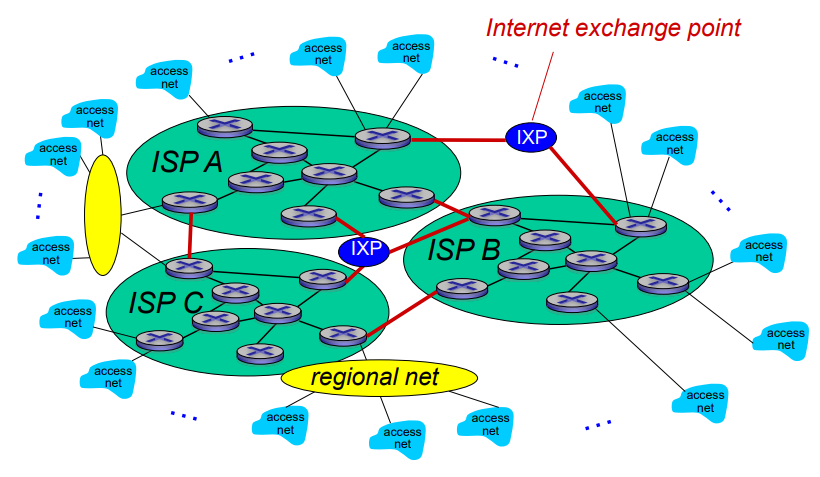
\includegraphics[width=0.6\linewidth]{internetstructure}}
\end{itemize}


\subsubsection{Network Edge (Access Network)}
\begin{itemize}
\item The access network is the network that physically
connects an end system to the first router on a path
from that end system to any distant end system.
\item E.g. Residential access networks, mobile access networks.
\end{itemize}
  
\subsubsection{Network Core}
\begin{itemize}
\item A mesh of interconnected routers.
\item Data is transmitted through network through:
\item \textbf{Circuit switching:} dedicated circuit per call
\item \textbf{Packet switching:} data sent through net in discrete “chunks"
\end{itemize}
  
\subsubsection{Circuit Switching}
\begin{itemize}
\item End-end resources are allocated to and reserved for “call”  between source \& dest:
\item call setup required, circuit-like (guaranteed) performance
\item circuit segment idle \textbf{silent periods} if not used by call (no sharing)
\item commonly used in traditional telephone network
\end{itemize}

\subsubsection{Packet Switching}
\begin{itemize}
\item Host sending function: breaks application message into smaller 
chunks, known as packets, of length $L$ bits. Then, transmits packets onto the link at transmission rate $R$.
\item Packets are passed from one router to the next, across links on path from source to destination.
\item link transmission rate is aka link capacity or \textbf{link bandwidth}
\item \textbf{Packet transmission delay} (time taken to transmit L-bit packet into Link) = $\frac{L}{R}$
\item \textbf{Store-and-forward}: entire packet must arrive at a router before it can be transmitted on the next link.
\end{itemize}


\subsubsection{Delay, Loss, Throughput}
Four sources of packet delay, suffered at each node, from source to destination. (\textbf{Total nodal delay})
\centerline{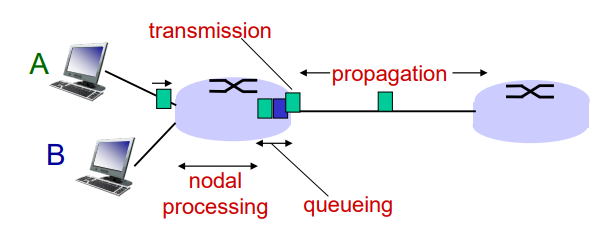
\includegraphics[width=0.6\linewidth]{totalnodaldelay}}
\begin{itemize}
\item \textbf{Nodal Processing Delay}: Time required to check for bit errors and determine output link. Typically $<$ msec.
\item \textbf{Queueing Delay}: Time waiting in queue for transmission, depends on earlier arrived packets. Typically $<$ msec. Additionally, possibility of
						packet loss if router queue full (buffer has reached finite capacity), and drops packet.
\item \textbf{Transmission Delay}: Time to push (last bit) of packet on wire. $d_{trans} = \frac{L}{R}$.
\item \textbf{Propagation Delay}: Time to propagate to next router. $d_{prop} = \frac{d}{s}$, where $d$ is length of physical link, $s$ propagation speed.
\item End to end packet delay is total time taken for packet to travel from source to destination, consisting of the 4 delays.
\item \textbf{Throughput}: How many bits can be transmitted per unit time, usually measured for end-to-end communication (as opposed to bandwidth for specific link).
\end{itemize}

\subsubsection{Internet Protocol Stack}
Protcols logically organised into 5 "layers" according to purpose. (Additionally presentation and session layers not included)
\begin{itemize}
\item \textbf{Application}: Where network applications and app-layer protocols reside. Packet here called message. \\ 
Examples: HTTP, SMTP, FTP
\item \textbf{Transport}: Transports app-layer messages between application endpoints. Packet here called segment.  \\
Examples: TCP, UDP
\item \textbf{Network}: Moves packets (datagrams) from one host to another. Includes IP protocol and other routing protocols.
\item \textbf{Link}: Moves packet from one node to another. Packet here called frame. \\
Example: Ethernet, WiFi
\item \textbf{Physical}: Moves individual bits within link-layer frame from one node to another. Link and transmission medium dependent.
\end{itemize}

\vfill \null
\columnbreak
%                              -----------------------------------------------------

\section{2. Application Layer}
\subsubsection{Principles of Network Applications}
\begin{itemize}
\item \textbf{Client-Server}: \\
• Server waits for incoming requests and provides required services to client. Easy scalability. \\
• Client initiates contact with server and requests service.
\item \textbf{Peer-To-Peer (P2P)}: \\
• No dedicated server, instead it relies on direct communication between pairs of intermittently connected hosts called peers. \\
• Self-scalability, each peer generates workload but adds service capacity by distributing files.
\end{itemize}

\subsubsection{Process Communication}
\begin{itemize}
\item \textbf{Socket}: A software interface that process uses to send messages and receive messages from network. Generally a combination of IP address and port number. 
\item \textbf{IP Address}: A 32-bit quantity, uniquely identifies host.
\item \textbf{Port Number}: A 16-bit integer used to identify a receiving process running in a host.
\end{itemize}

\subsubsection{Requirements of Transport Service}
\begin{itemize}
\item \textbf{Reliable Data Transfer}: Data to sent correctly and completely vs. loss-tolerant.
\item \textbf{Throughput}: Bandwidth-sensitive apps may need guaranteed throughput of r bits/sec. 
\item \textbf{Timing/Delay}: Real-time applications generally require low delays to be effective.
\item \textbf{Security}: Encryption, data integrity, authentication.
\end{itemize}

\subsubsection{Transport Layer Protocols}
Two main protocols for the Internet. \\
\begin{itemize}
\item \textbf{Transmission Control Protocol (TCP)} \\
• Reliable data transfer, Connection-oriented service: A handshake required.\\
• Flow control, Congestion control: Throttle sender when network overloaded \\
• Security: Can be enhanced at the app layer with Secure Sockets Layer \\
• Does not provide: Timing and throughput guarantee
\item \textbf{User Datagram Protocol (UDP)} \\
• Unreliable data transfer \\
• Connectionless: No handshake \\
• No flow control, no congestion control \\
• Does not provide: Timing and throughput guarantee, security.
\end{itemize}

\subsubsection{Application-Layer Protocols} 
An application-layer protocol defines:
\begin{itemize}
\item Types of messages exchanged, e.g. request and response messages.
\item Syntax of message types, e.g. fields and how they are delineated.
\item Semantics of the fields, i.e. what the information means.
\item Rules for when and how to send a message and respond to messages.
\end{itemize}

\subsection{Web \& HTTP}
\begin{itemize}
\item \textbf{Webpage}: Consists of base HTML files and referenced objects. Addressable by URL.
\item URL made up of hostname as well as path name. (E.g. http://www.comp.nus.edu.sg/~cs2105/img/doge.jpg)
\item \textbf{HyperText Transfer Protocol} is Web’s app-layer protocol.
\item \textbf{Client-server model:} Client requests, receives and displays Web objects, server is Web server that sends objects in response.
\item \textbf{Stateless}: server maintains no information about clients, and \textbf{Reliable}: Over TCP.
\item \textbf{Three-way Handshake}: Client sends small TCP segment to ask for connection, server acknowledges and responds, client acknowledges and sends it back with request message.
\end{itemize}

\subsubsection{HTTP versions}
\begin{itemize}
\item \textbf{RTT}: Round trip time, time taken for packet to travel from server and back to client, does not include transmission delay.
\item \textbf{Non-persistent HTTP}: Response time = $2 *$ RTT$+$ file transmission time (per object)
\item \textbf{Persistent HTTP}: Server leaves connection open after sending response, subsequent HTTP sent over same TCP connection. Also uses pipelining, send requests back to back.
\end{itemize}
\smallskip
\centerline{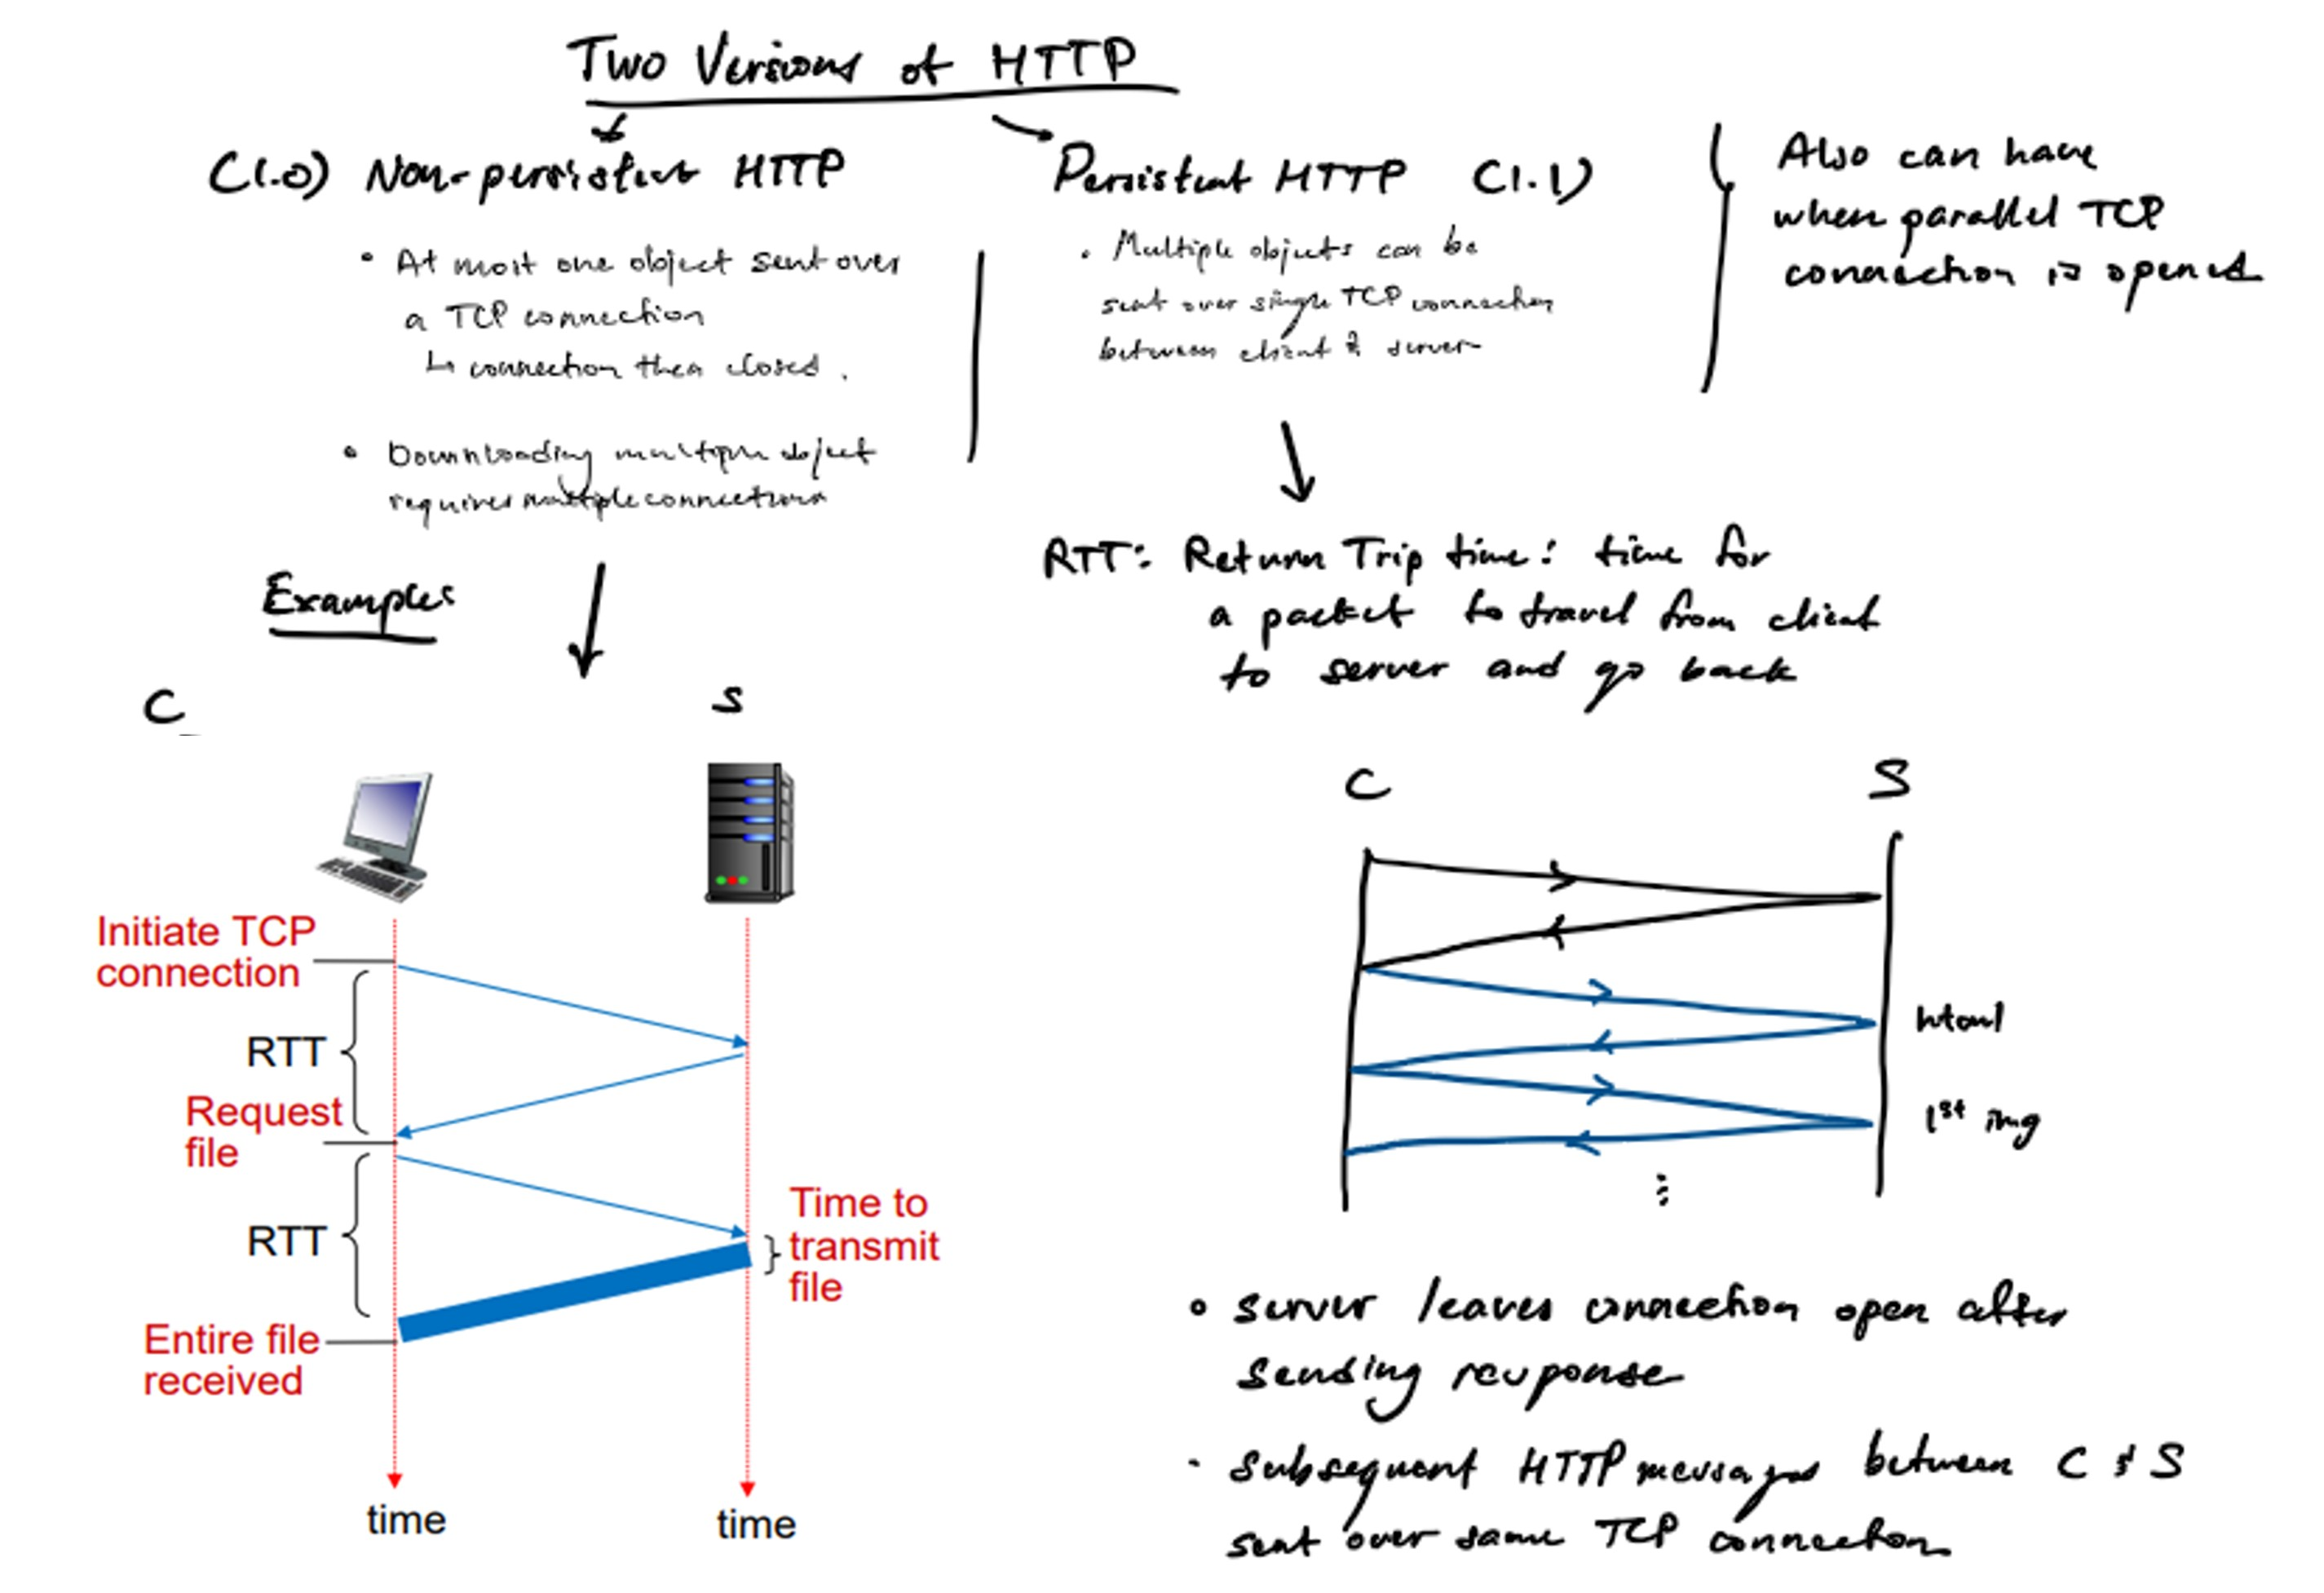
\includegraphics[width=1\linewidth]{HTTPmodes}}
\medskip
\subsubsection{HTTP Request}
\centerline{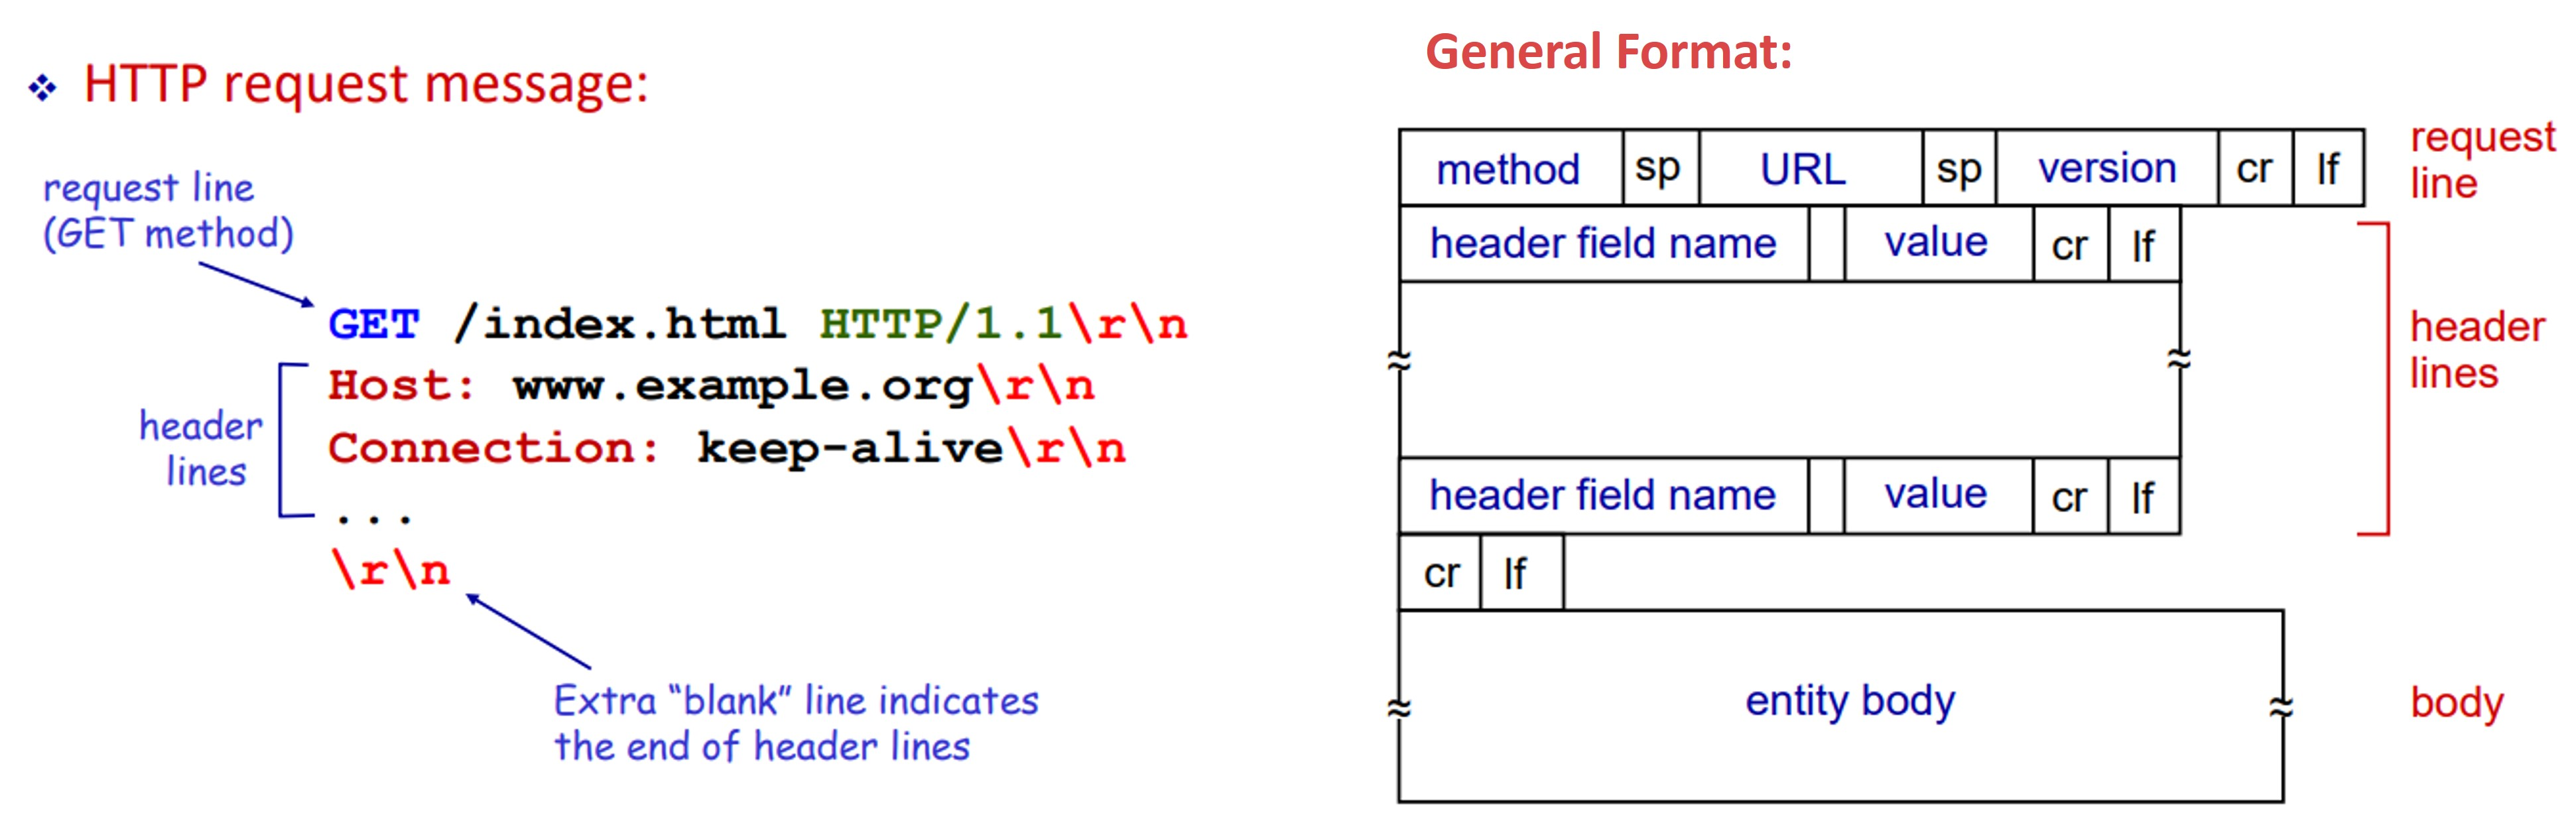
\includegraphics[width=1\linewidth]{HTTPrequest}}
\begin{itemize}
\item \textbf{HTTP 1.0 Methods}: GET (gets object), POST (posts form data), HEAD (gets header without body).
\item \textbf{HTTP 1.1 Methods}: GET, POST, HEAD, PUT (uploads file to path specified), DELETE
\end{itemize}
\medskip
\subsubsection{HTTP Response}
\centerline{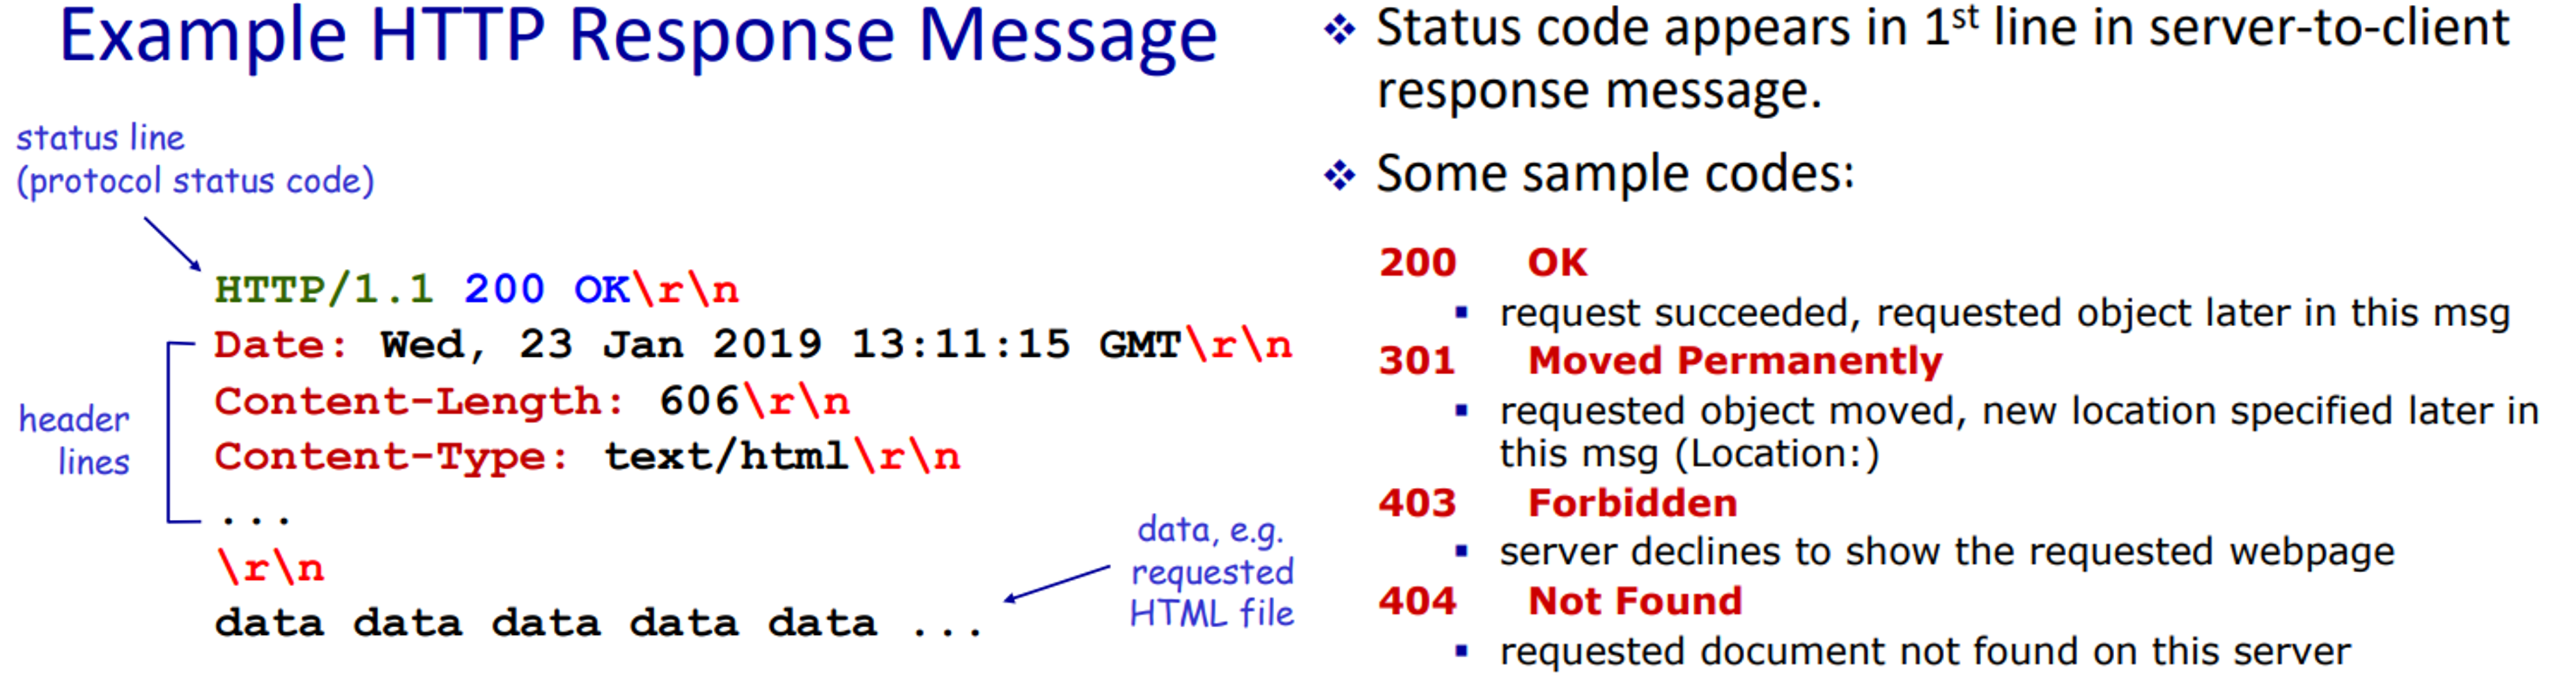
\includegraphics[width=1\linewidth]{HTTPresponse}}

\vfill \null
\columnbreak

\subsubsection{Cookies}
\begin{itemize}
\item HTTP is designed to be “stateless”, server maintains no information about past client requests. 
\item Good to maintain states over multiple transactions, e.g. shopping carts
\item \textbf{Cookie}: http messages carry “state”: \\
1) cookie header field of HTTP req/res messages \\ 
2) cookie file kept on user host, managed by browser\\
3) back-end database at Web site
\item \textbf{Conditional GET}: In cache, specify date of cached copy in HTTP request. Server response contains no object if cached copy is up to date.
\end{itemize}
\medskip
\centerline{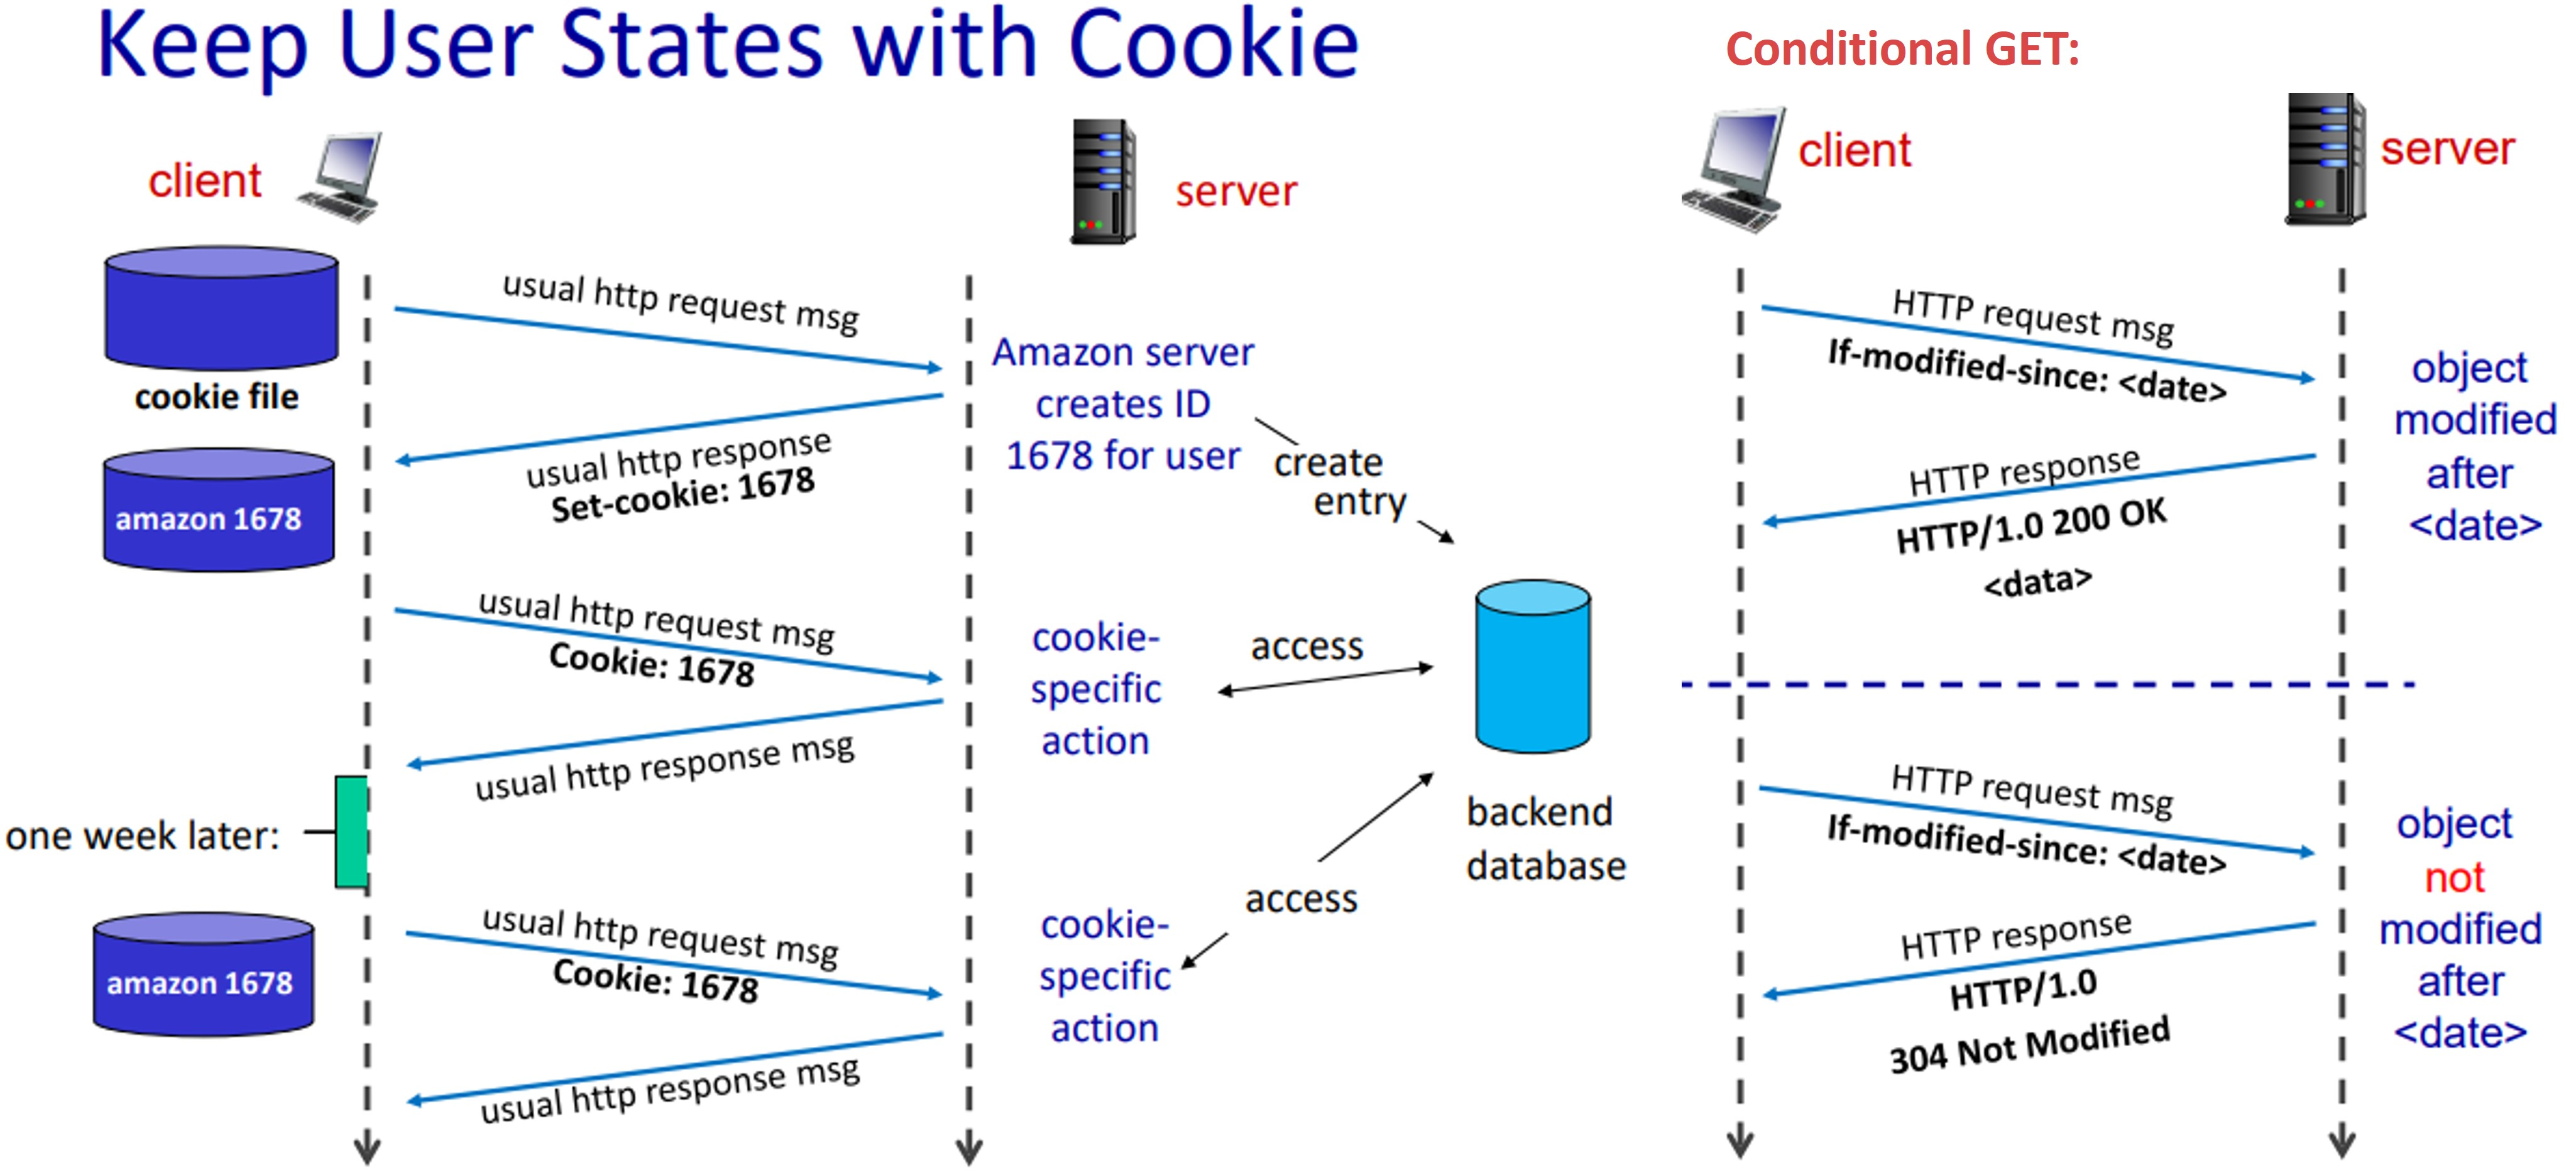
\includegraphics[width=1\linewidth]{HTTPcookies}}


\subsubsection{Domain Name System}
DNS translates between hostname and IP addresses. Client must carry out a DNS query to determine the 
IP address corresponding to the server name.
\begin{itemize}
\item \textbf{DNS: Resource Records (RR)}
\centerline{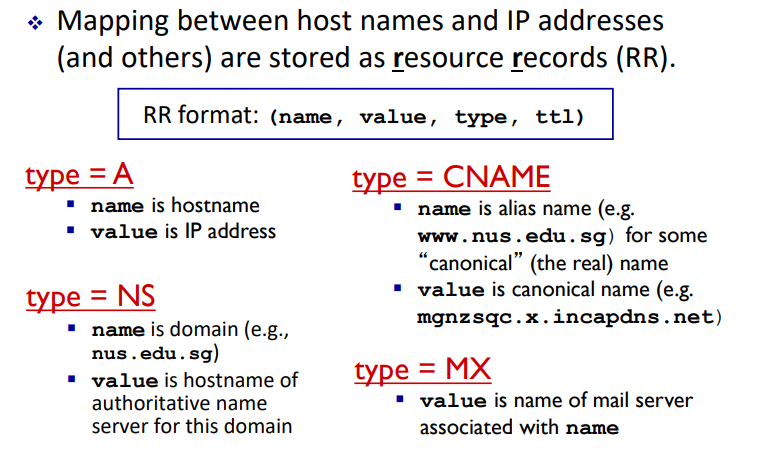
\includegraphics[width=1\linewidth]{DNSrr}}
\item \textbf{Distributed, Hierarchical Database}: DNS servers form hierarchy to distribute mappings. Contains root servers (for Top Level Domain TLD servers), 
								TLD servers (e.g. uk, sg), Authoritative servers.
\item Local DNS servers have local cache, acts as proxy, forward query into hierarchy if answer not found locally.
\item \textbf{DNS Caching}: Cache mapping, which expires after some time (TTL: time to live). 
\item DNS runs over \textbf{UDP}.
\end{itemize}

\subsubsection{DNS Name Resolution}
\centerline{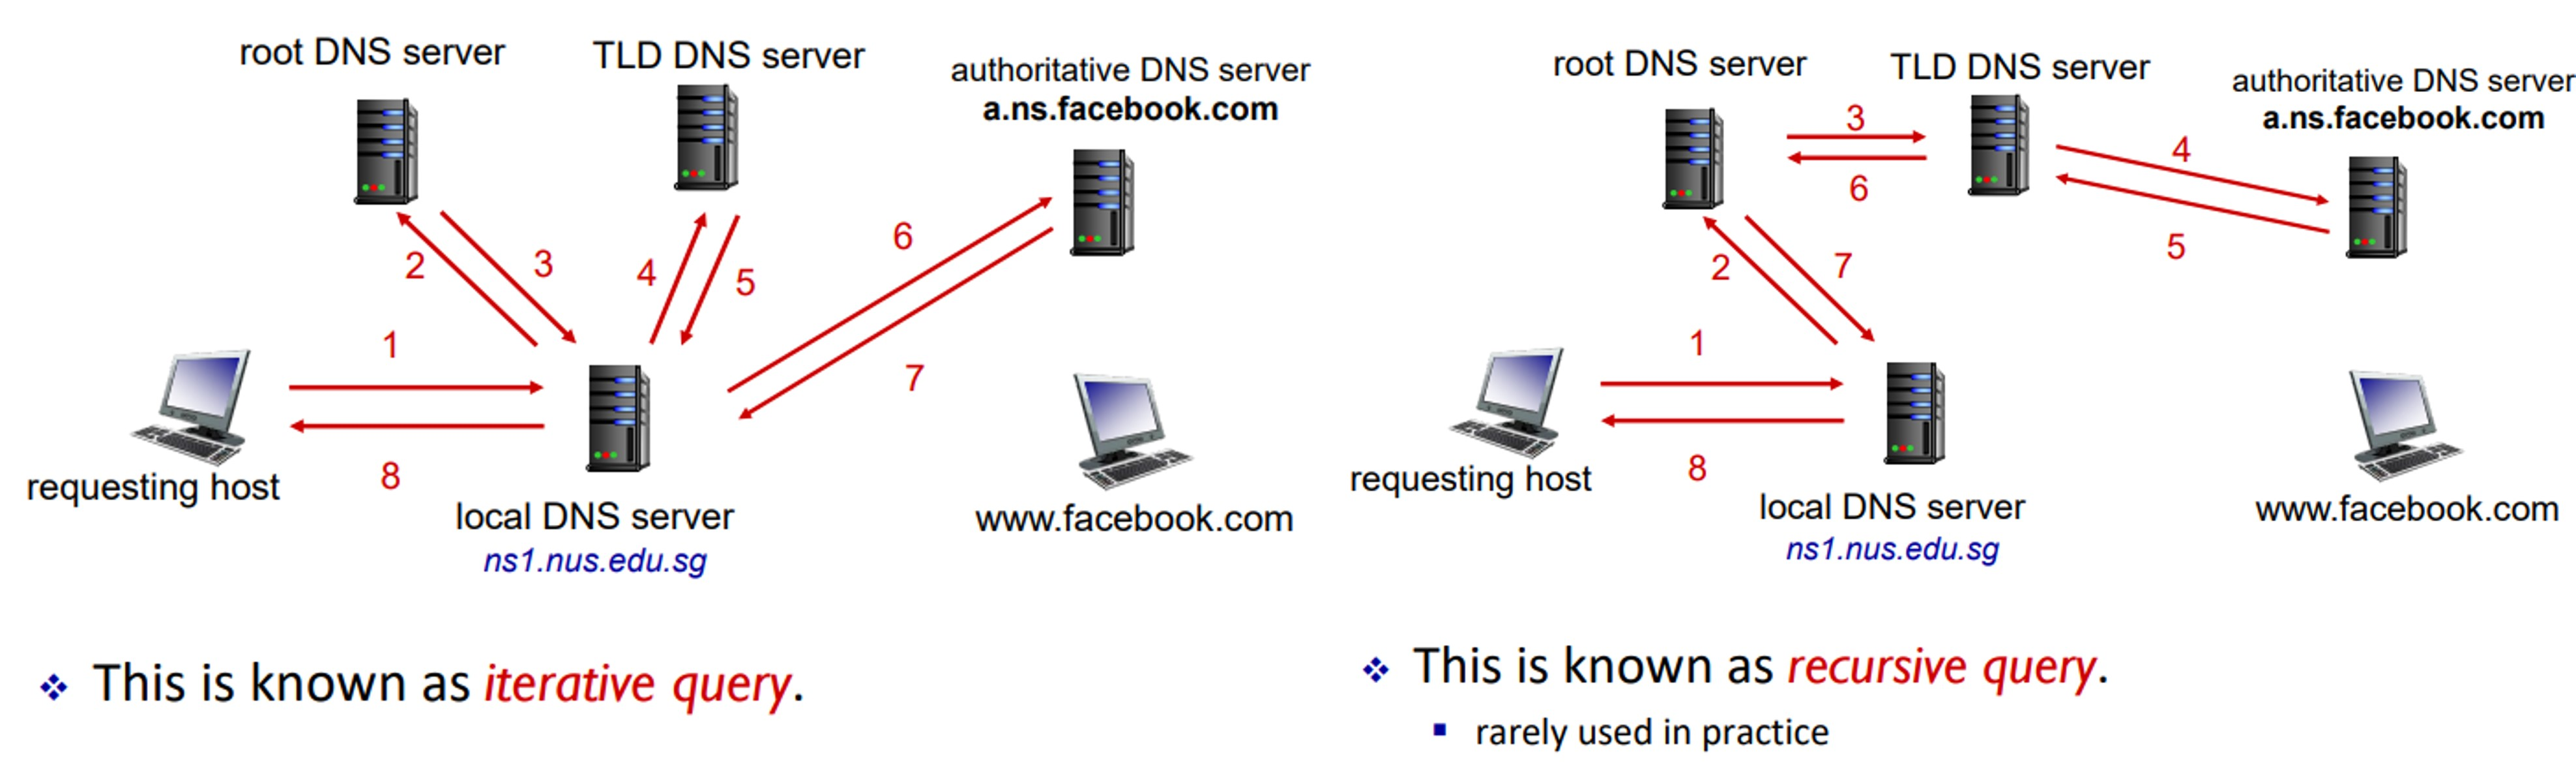
\includegraphics[width=1\linewidth]{DNSname}}
\medskip

\subsection{Socket Programming}
Applications treat the Internet as black box, send/receive message through sockets.
\begin{itemize}
\item Two types of sockets
\item \textbf{TCP}: reliable, byte stream-oriented socket
\item \textbf{UDP}: unreliable datagram socket
\end{itemize}

\subsubsection{UDP vs. TCP Socket}
\begin{itemize}
\item \textbf{UDP Socket:}Sender attach des IP address + port no. to each packet. (OS inserts add. info source IP and port). 
Receiver extracts sender IP + port number from packet.
\item \textbf{TCP Socket:} Attempts to establish TCP connection to server first. Server TCP contacted creates new socket to communicate with client, allows server to talk with multiple clients individually.
\end{itemize}
\centerline{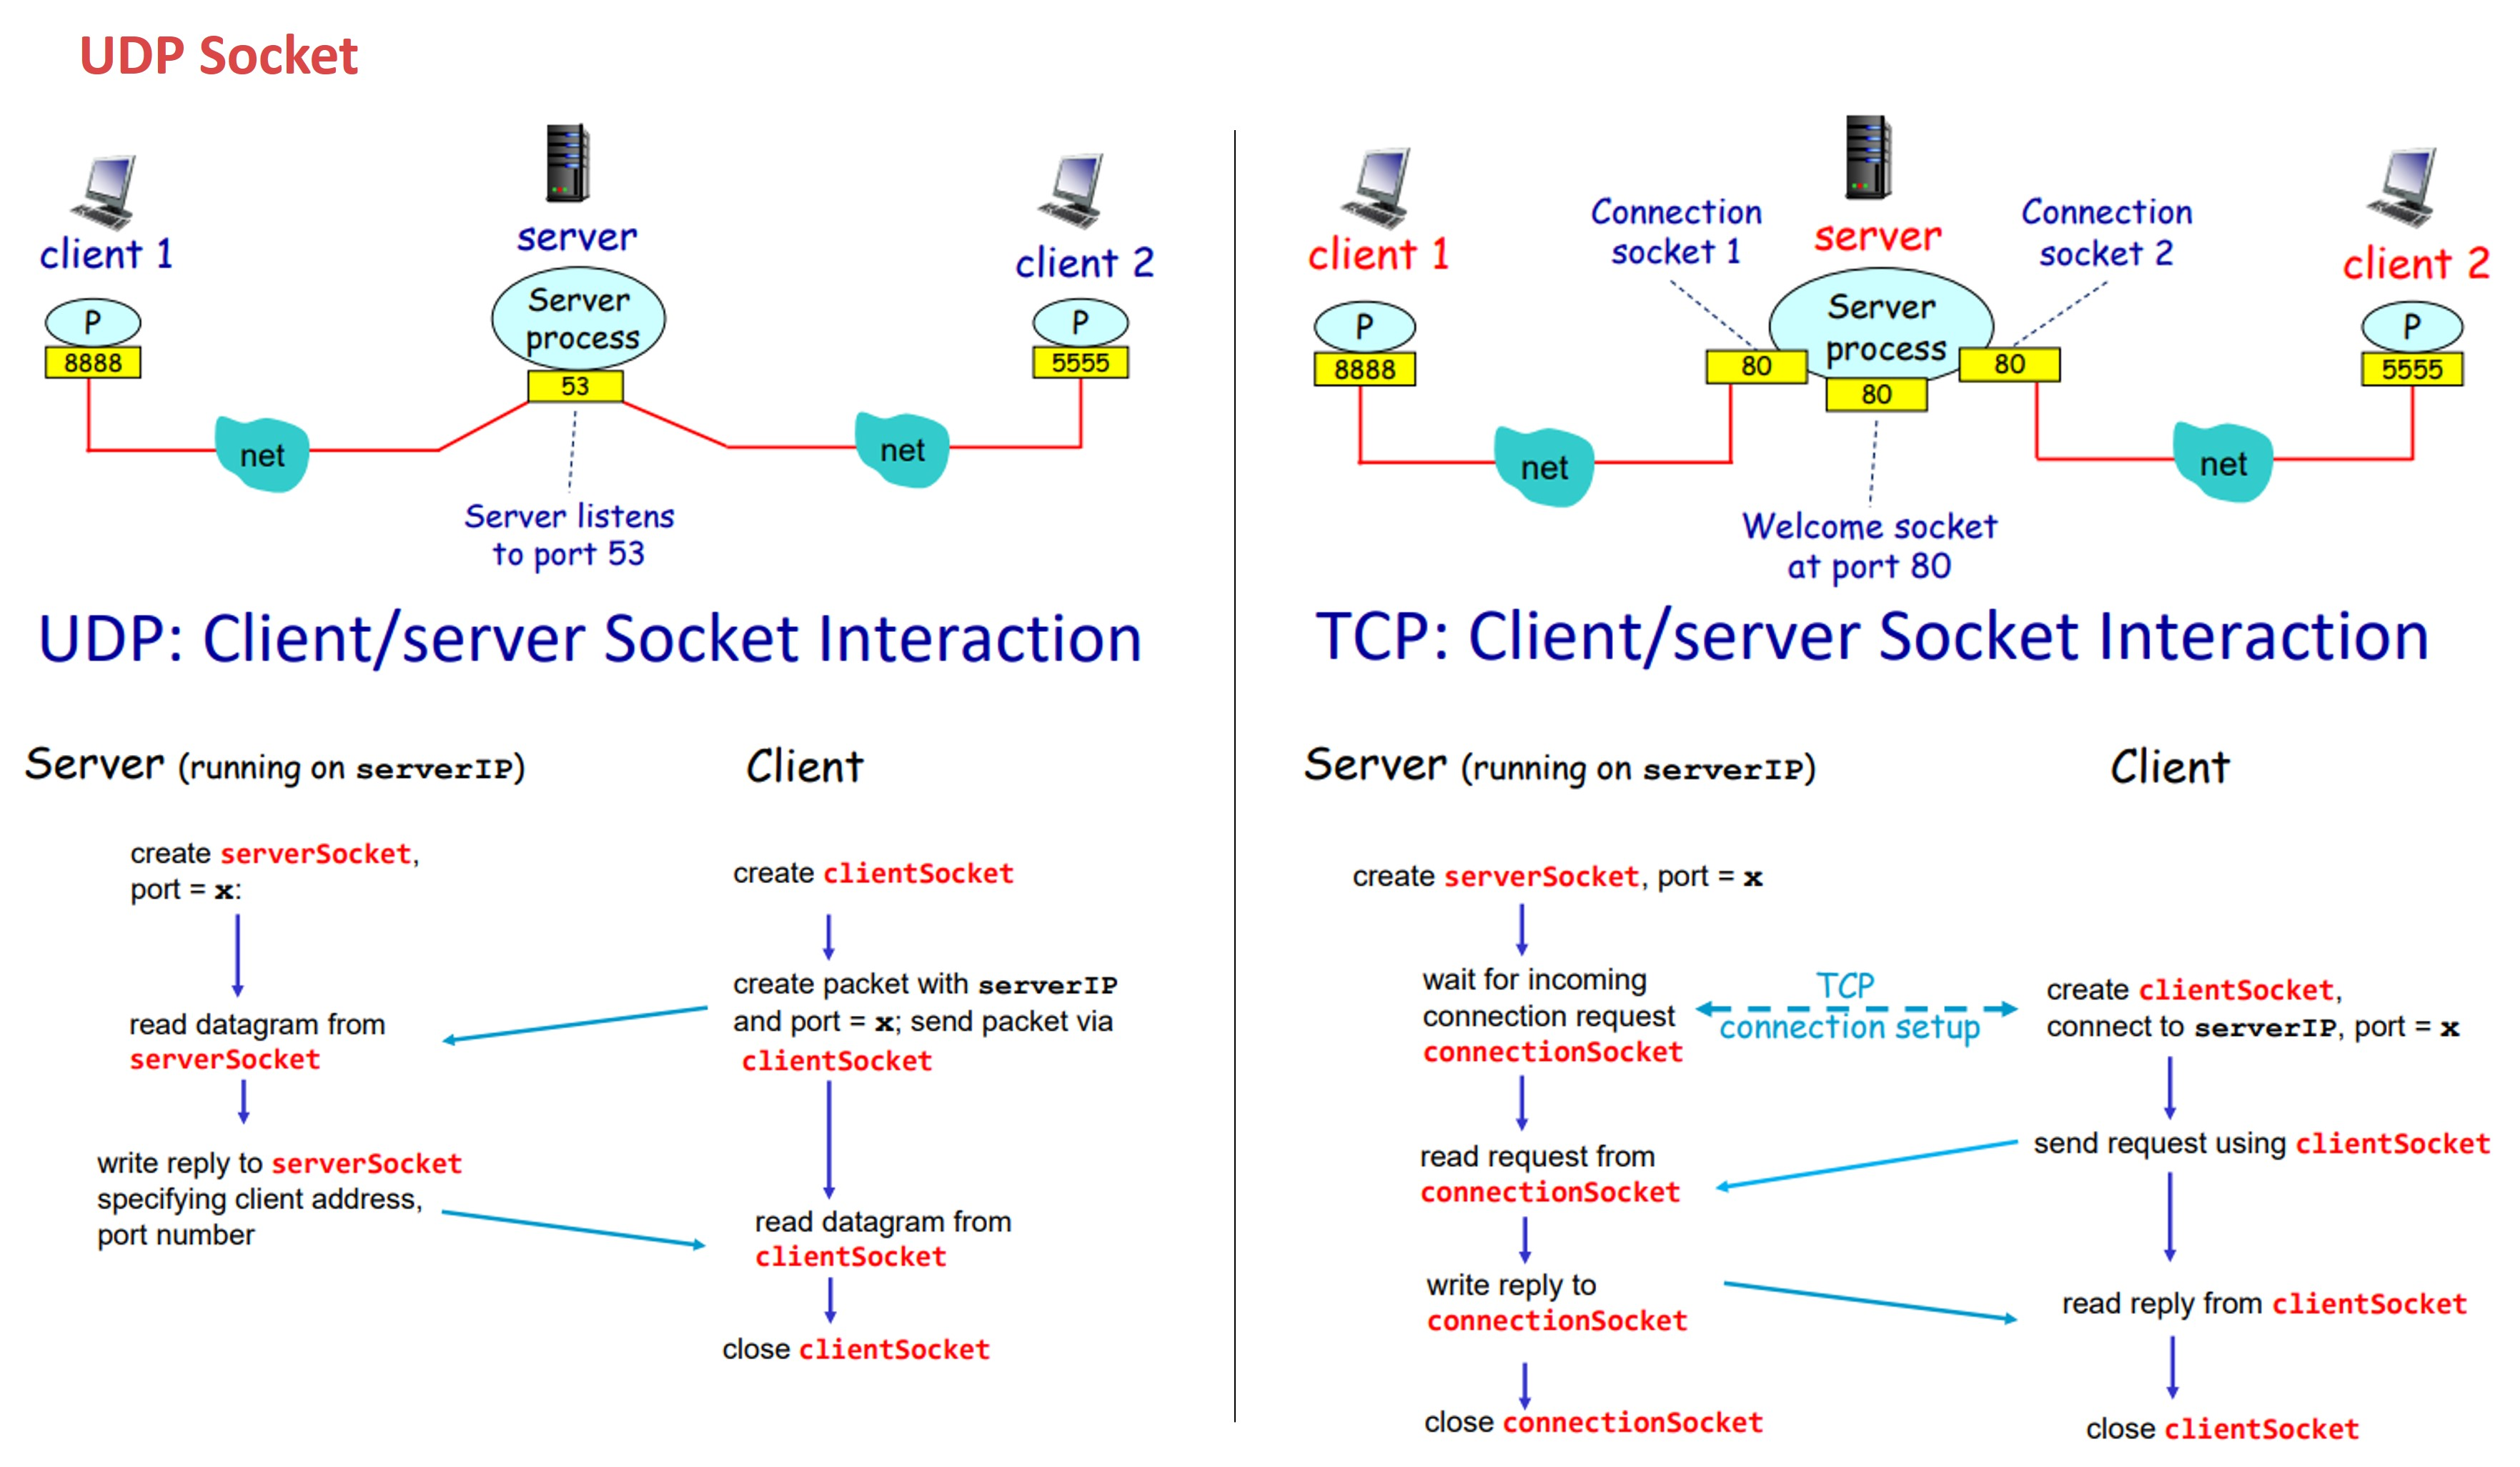
\includegraphics[width=1\linewidth]{socket}}
\begin{itemize}
\item \textbf{TCP vs. UDP Differences}
\item In TCP, two processes communicate as if pipe between them. The pipe remains in place until one of two processes closes it. Sending process doesn’t need to attach a destination IP 
/ port number to the bytes in sending attempt as the logical pipe has been established
\item In UDP, programmers need to form UDP datagram packets explicitly and attach destination IP address / port number to every packet.
\end{itemize}

\vfill \null
\columnbreak

\section{3. Transport}
\subsubsection{Transport Layer Services}
\begin{itemize}
\item Transport layer protocols run in hosts.
\item Sender side: breaks app message into segments (as 
needed), passes them to network layer (aka IP layer).
\item Receiver side: reassembles segments into message, 
passes it to app layer.
\item Packet switches (routers) in between: only check 
destination IP address to decide routing.
running on different hosts
\end{itemize}

\subsubsection{Transport and Network Layer}
\begin{itemize}
\item \textbf{Transport} layer takes care of logical communication
between \textbf{processes}. 
\item \textbf{Network} layer takes care of
logical communication between \textbf{hosts}. (best-effort, unreliable)
\item \textbf{IP Datagram}: Contains source and dest IP addresses, carries one transport layer segment that contains source and dest port numbers.
\end{itemize}



\section{UDP: Connectionless Transport}
\begin{itemize}
\item UDP adds very little service on top of IP.
\item \textbf{Multiplexing at sender}: UDP gathers data, forms packets, passes to IP.
\item \textbf{De-multiplexing at receiver}: UDP receives packets from lower layer, checks dest port, and dispatches them to right processes.
\item \textbf{Unreliable}: UDP transmission used by loss tolerant and rate sensitive apps.
\centerline{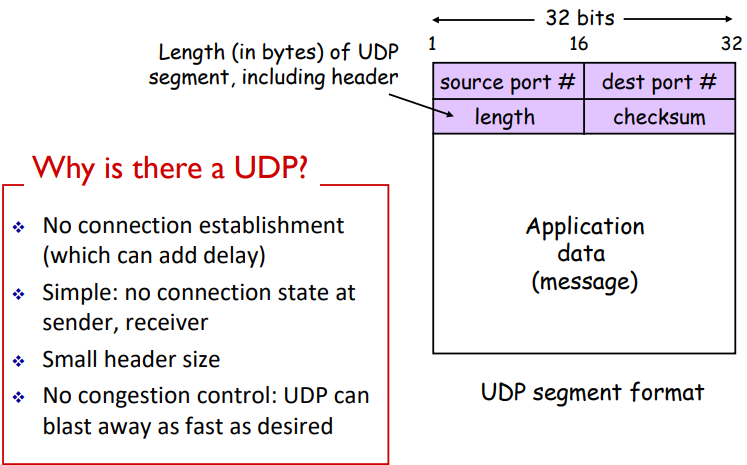
\includegraphics[width=0.8\linewidth]{udpheader}}
\end{itemize}

\subsubsection{UDP Checksum}
\begin{itemize}
\item Allows for error detection, but not correction. May be bit errors when segments are stored and passed in router memory.
\item  Treat UDP segment as a sequence of 16-bit integers.
\item Apply binary addition on every 16-bit integer (checksum field currently 0).
\item If carry from MSB, add 1 to result (wrap).
\item Compute 1’s complement to get UDP checksum.
\end{itemize}

\subsubsection{Principles of Reliable Data Transfer (rdt)}
We need to build a reliable transport layer protocol
on top of unreliable communication.
\begin{itemize}
\item Factors: \textbf{Packet corruption, Packet loss, Packet reordering, Packet (Long) Delay.}
\item Finite State Machines to describe protocol.
\end{itemize}
\medskip
Reliable Data Transfer: \textbf{Service Model}
\centerline{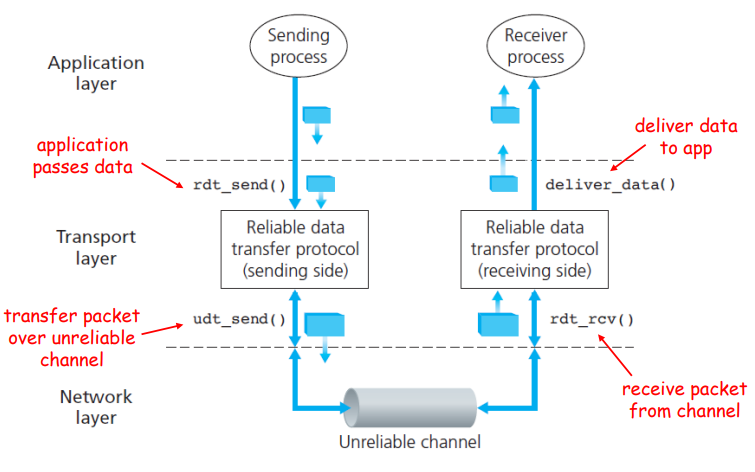
\includegraphics[width=0.8\linewidth]{rdtmodel}}

\subsubsection{rdt 1.0 (Perfectly Reliable)}
\begin{itemize}
\item Assumption: Underlying channel perfectly reliable.
\item Sender creates packet and sends, Receiver extracts and deliver data to application.
\end{itemize}

\subsubsection{rdt 2.0 (Corruptable Data)}
\begin{itemize}
\item Assumption: Underlying channel may flip bits. Use \textbf{stop and wait} (for receiver response) protocol. 
\item Receiver uses checksum to detect bit errors, sends NAK if corrupted. Sender resends if NAK received.
\item \textbf{Problem: If ACK or NACK corrupted}, no guaranteed way to recover. If packet resent, the receiver will not know it’s a duplicate.
\end{itemize}

\subsubsection{rdt 2.1}
\begin{itemize}
\item Add \textbf{sequence number to packet}, alternate 1 \& 0. Sequence number detects duplicates. 
\item Same as rdt2.0, but receiver knows if it is duplicate.
\end{itemize}
\medskip
\centerline{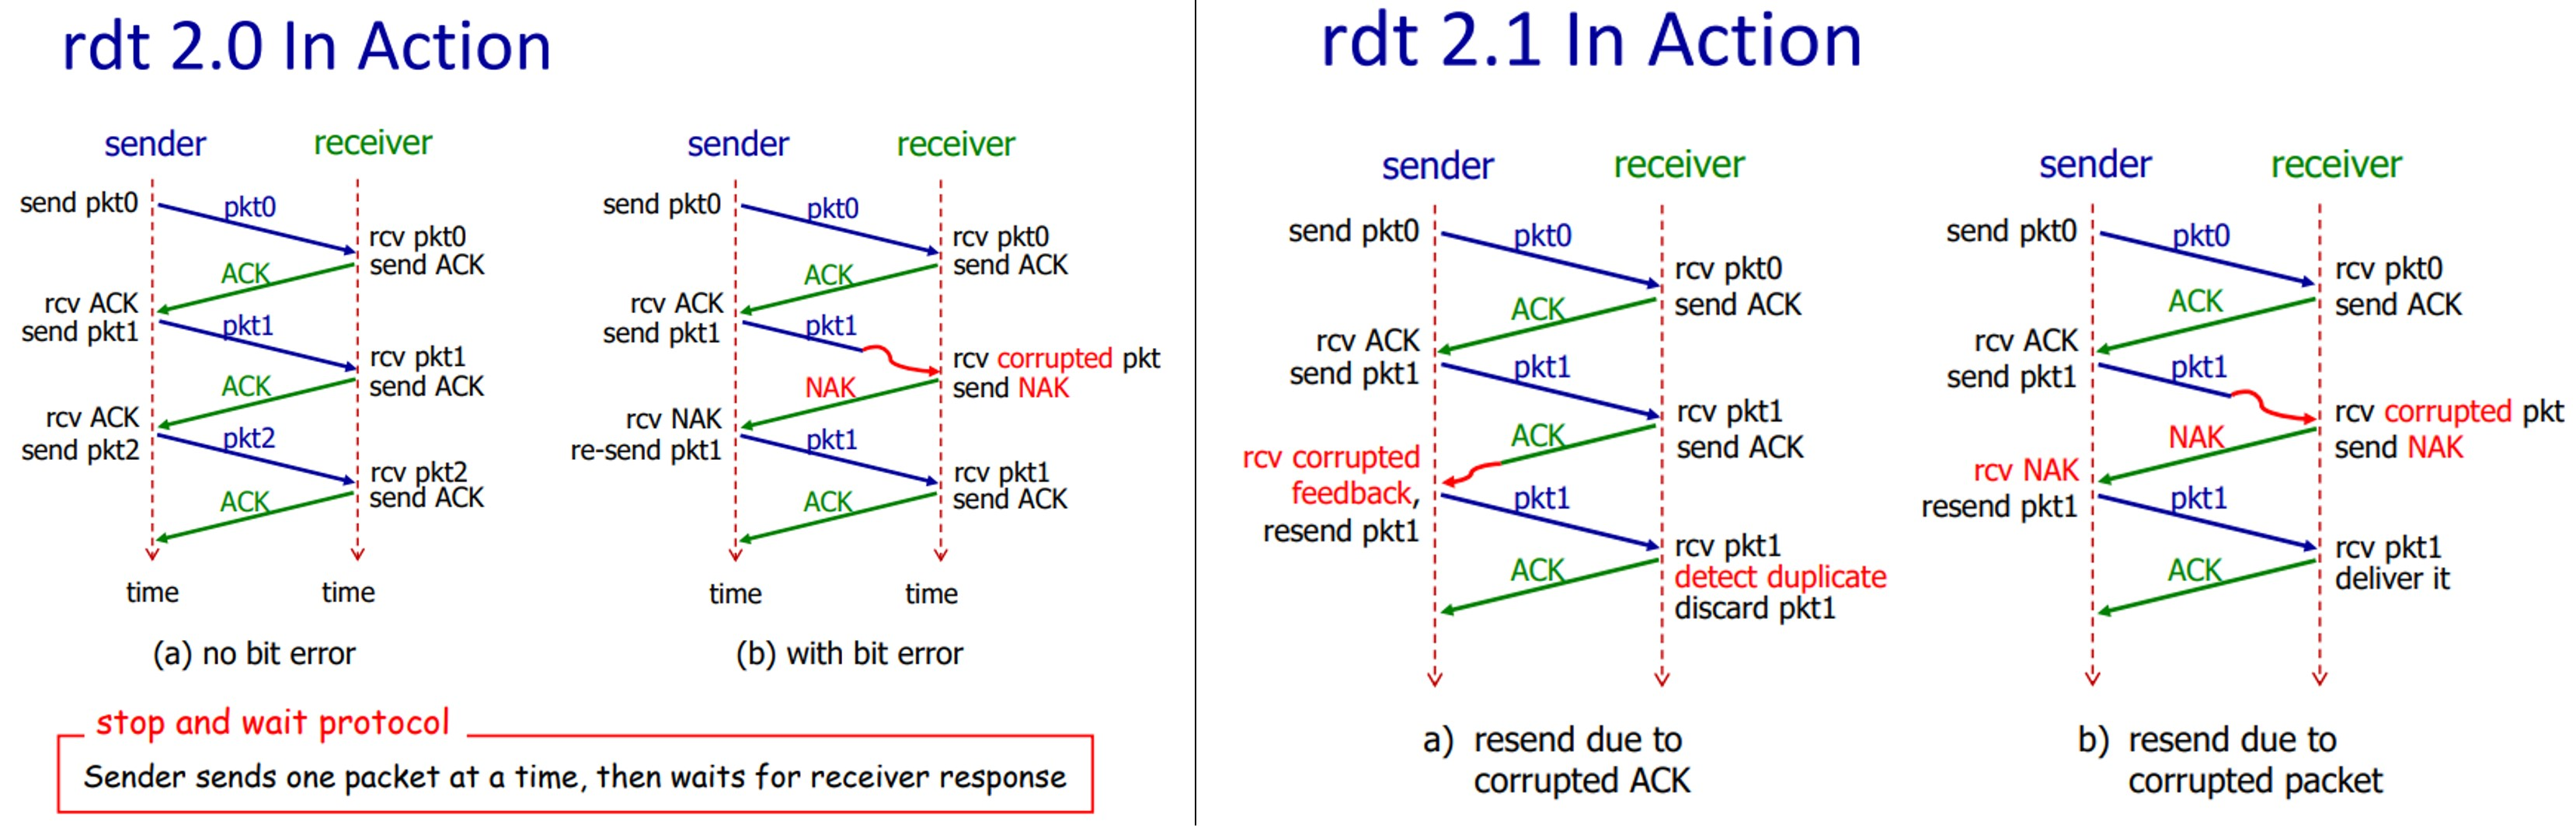
\includegraphics[width=1\linewidth]{rdt2.0-1}}

\subsubsection{rdt 2.2}
\begin{itemize}
\item \textbf{Use ACK of last packet sequence number for NAK.}  
\item Receiver explicitly include seq. no, duplicate ACKs results in retransmit current pkt.
\end{itemize}
\smallskip
\centerline{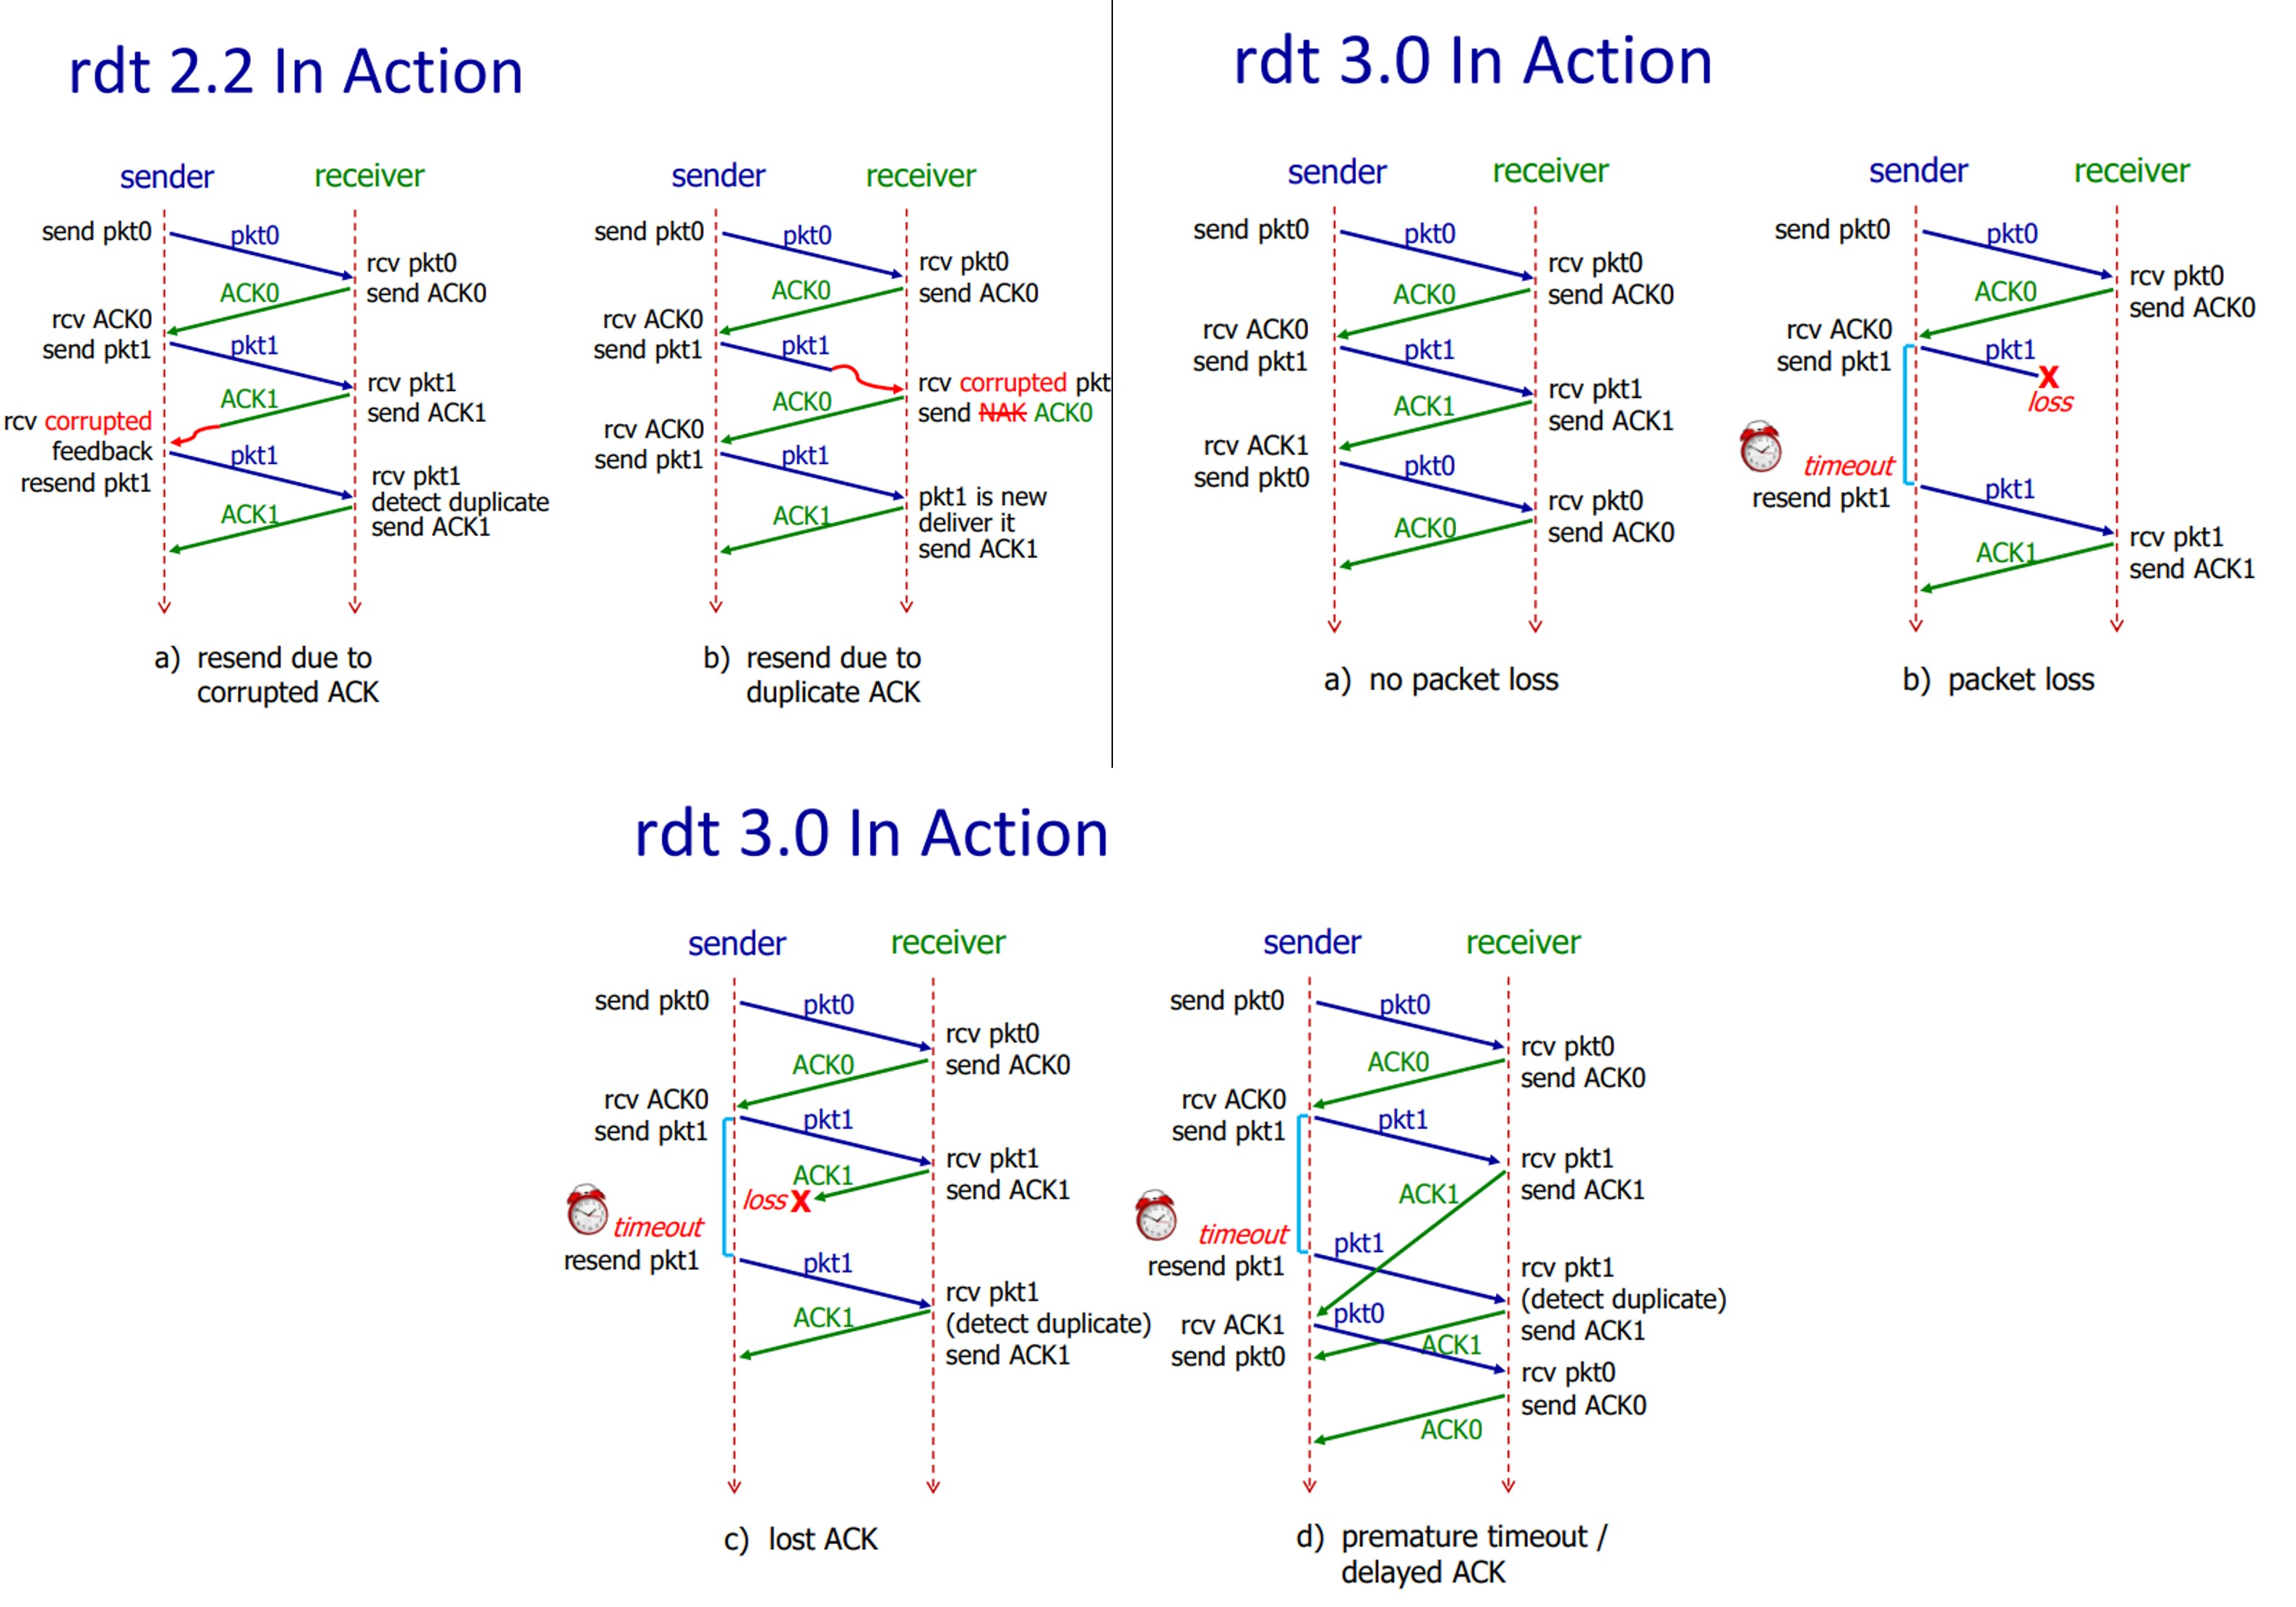
\includegraphics[width=1\linewidth]{rdt2.2-3}}

\subsubsection{rdt 3.0 (Corruptable, Lossy, Delay)}
\begin{itemize}
\item Assume corruption, packet loss/delay, no re-order. 
\item To detect packet loss, use \textbf{sender timeout}. Sender retransmits if no ACK received till timeout.
\item  If packet/ACK just delayed, retransmission may generate duplicates but receiver can use seq. no. to detect.
\item \textbf{rdt 3.0 performance}: Utilisation rate of sender low. For RTT 30ms, $L$ = 8000b, link 1GBps, $d_{trans}$ = 0.008ms, send 8000 bits per 30.008ms. Utilisation 0.027\%.
\item Stop and Wait limits use of physical resources.
\end{itemize}

\subsubsection{Pipelining}
\begin{itemize}
\item  \textbf{Pipelined Protocols}: sender allows multiple, “in-flight”, yet to-be-acknowledged packets. \\
• range of sequence numbers must be increased \\
• buffering at sender and/or receiver
\item Number of packets sent at once is called \textbf{window size}.
\item \textbf{Benchmarked Pipelined Protocols}: Go-Back-N (GBN), Selective Repeat (SR).
\item Assumption of corruption, packet loss / delay.
\end{itemize}

\subsubsection{Go-back-N}
\begin{itemize}
\item Sliding window, slides forward only when ACK received for the leftmost packet in window.
\item Requires $k$ bits in packet header for $2^k$ sequence number.
\item Sender keeps only 1 timer for oldest unACKed packet.
\item Receiver only accepts ACK packets that arrive in order, \underline{discards} out of order packets ACK last in-order sequence number. (cumulative ACK).
\end{itemize}
\smallskip
\centerline{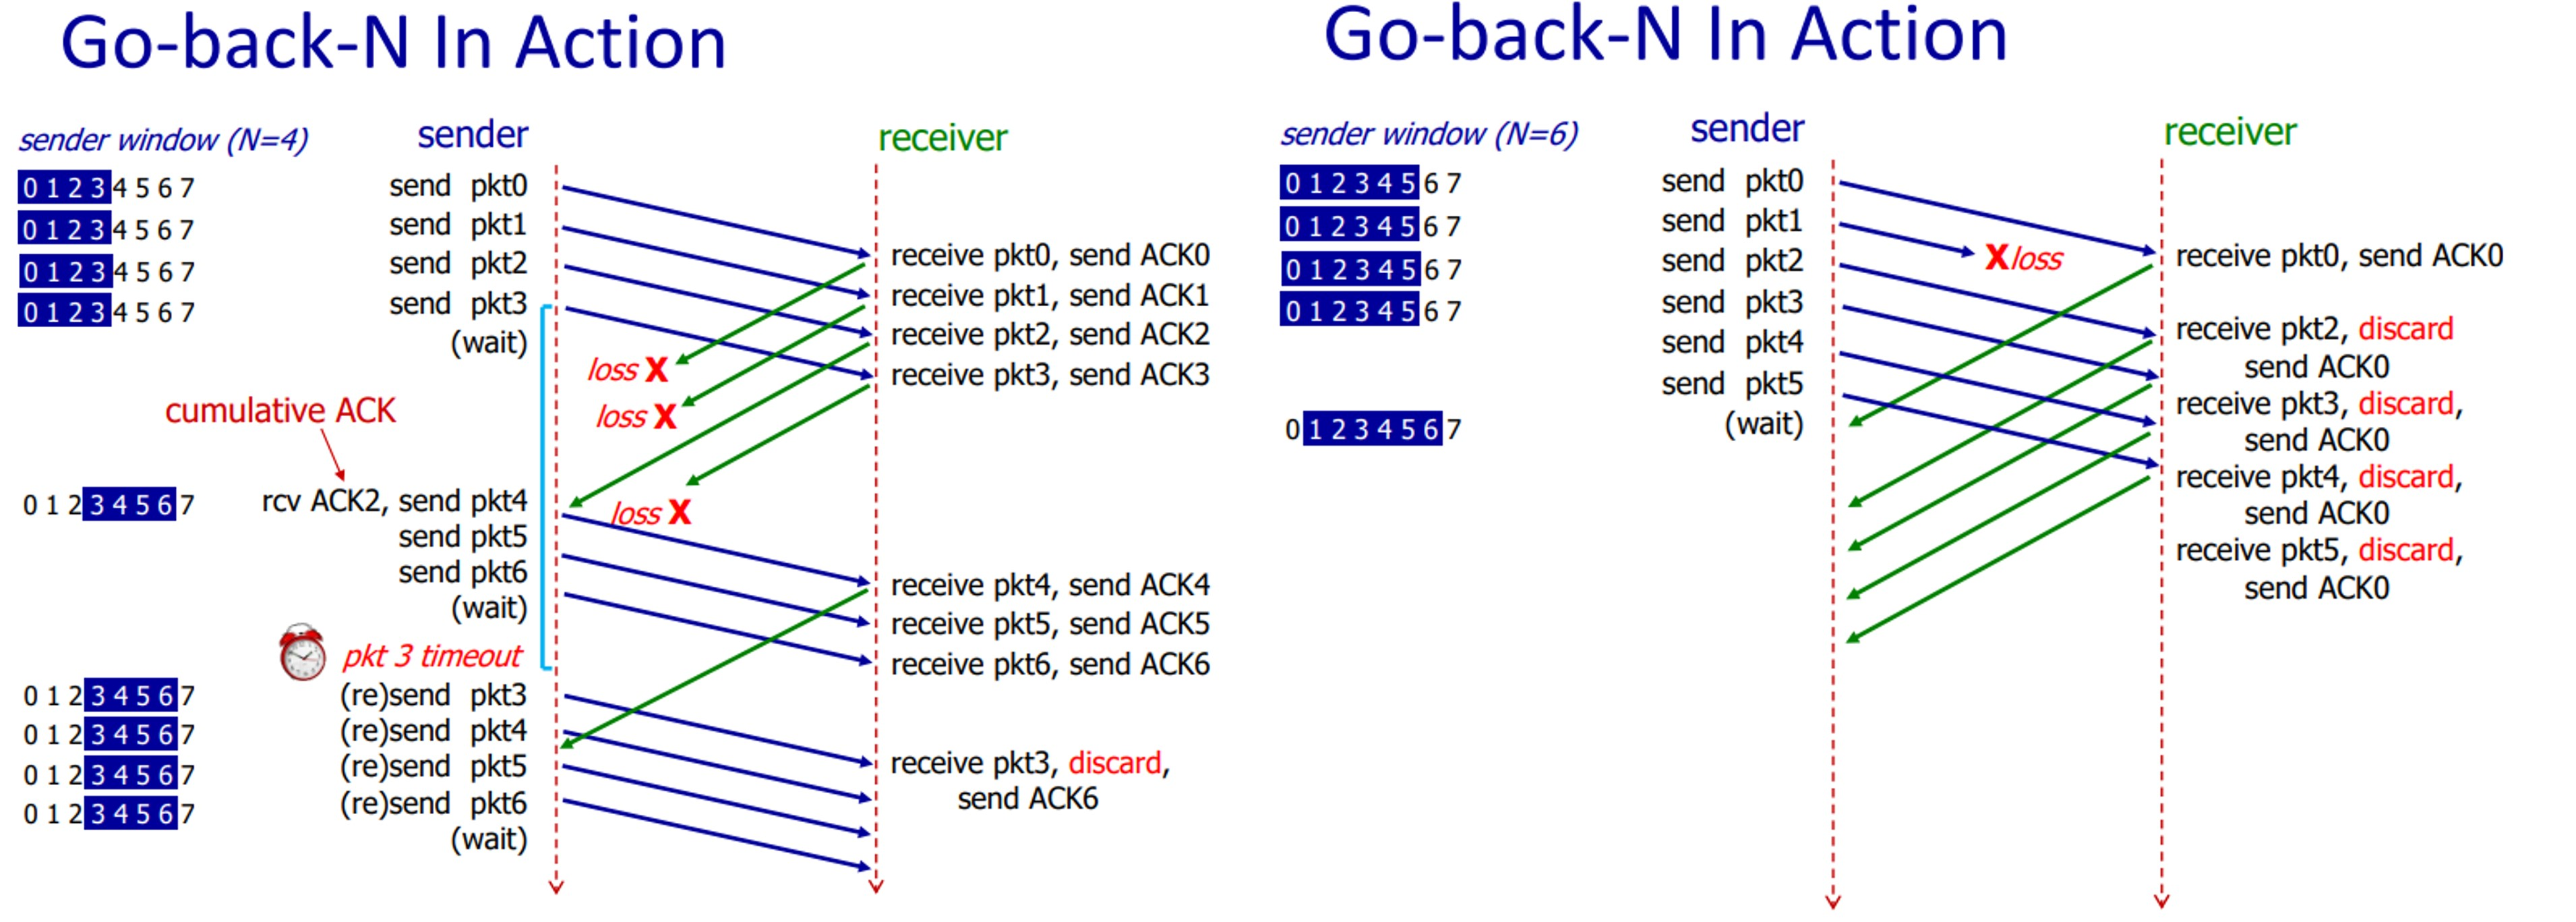
\includegraphics[width=1\linewidth]{gobackn}}

\subsubsection{Selective Repeat}
\begin{itemize}
\item Receiver individually acknowledges all correctly received packets.
\item Buffers out-of-order packets, for eventual in-order delivery to upper layer.
\item Sender maintains timer for each unACKed packet, When timer expires, retransmit only unACKed packet.
\end{itemize}
\smallskip
\centerline{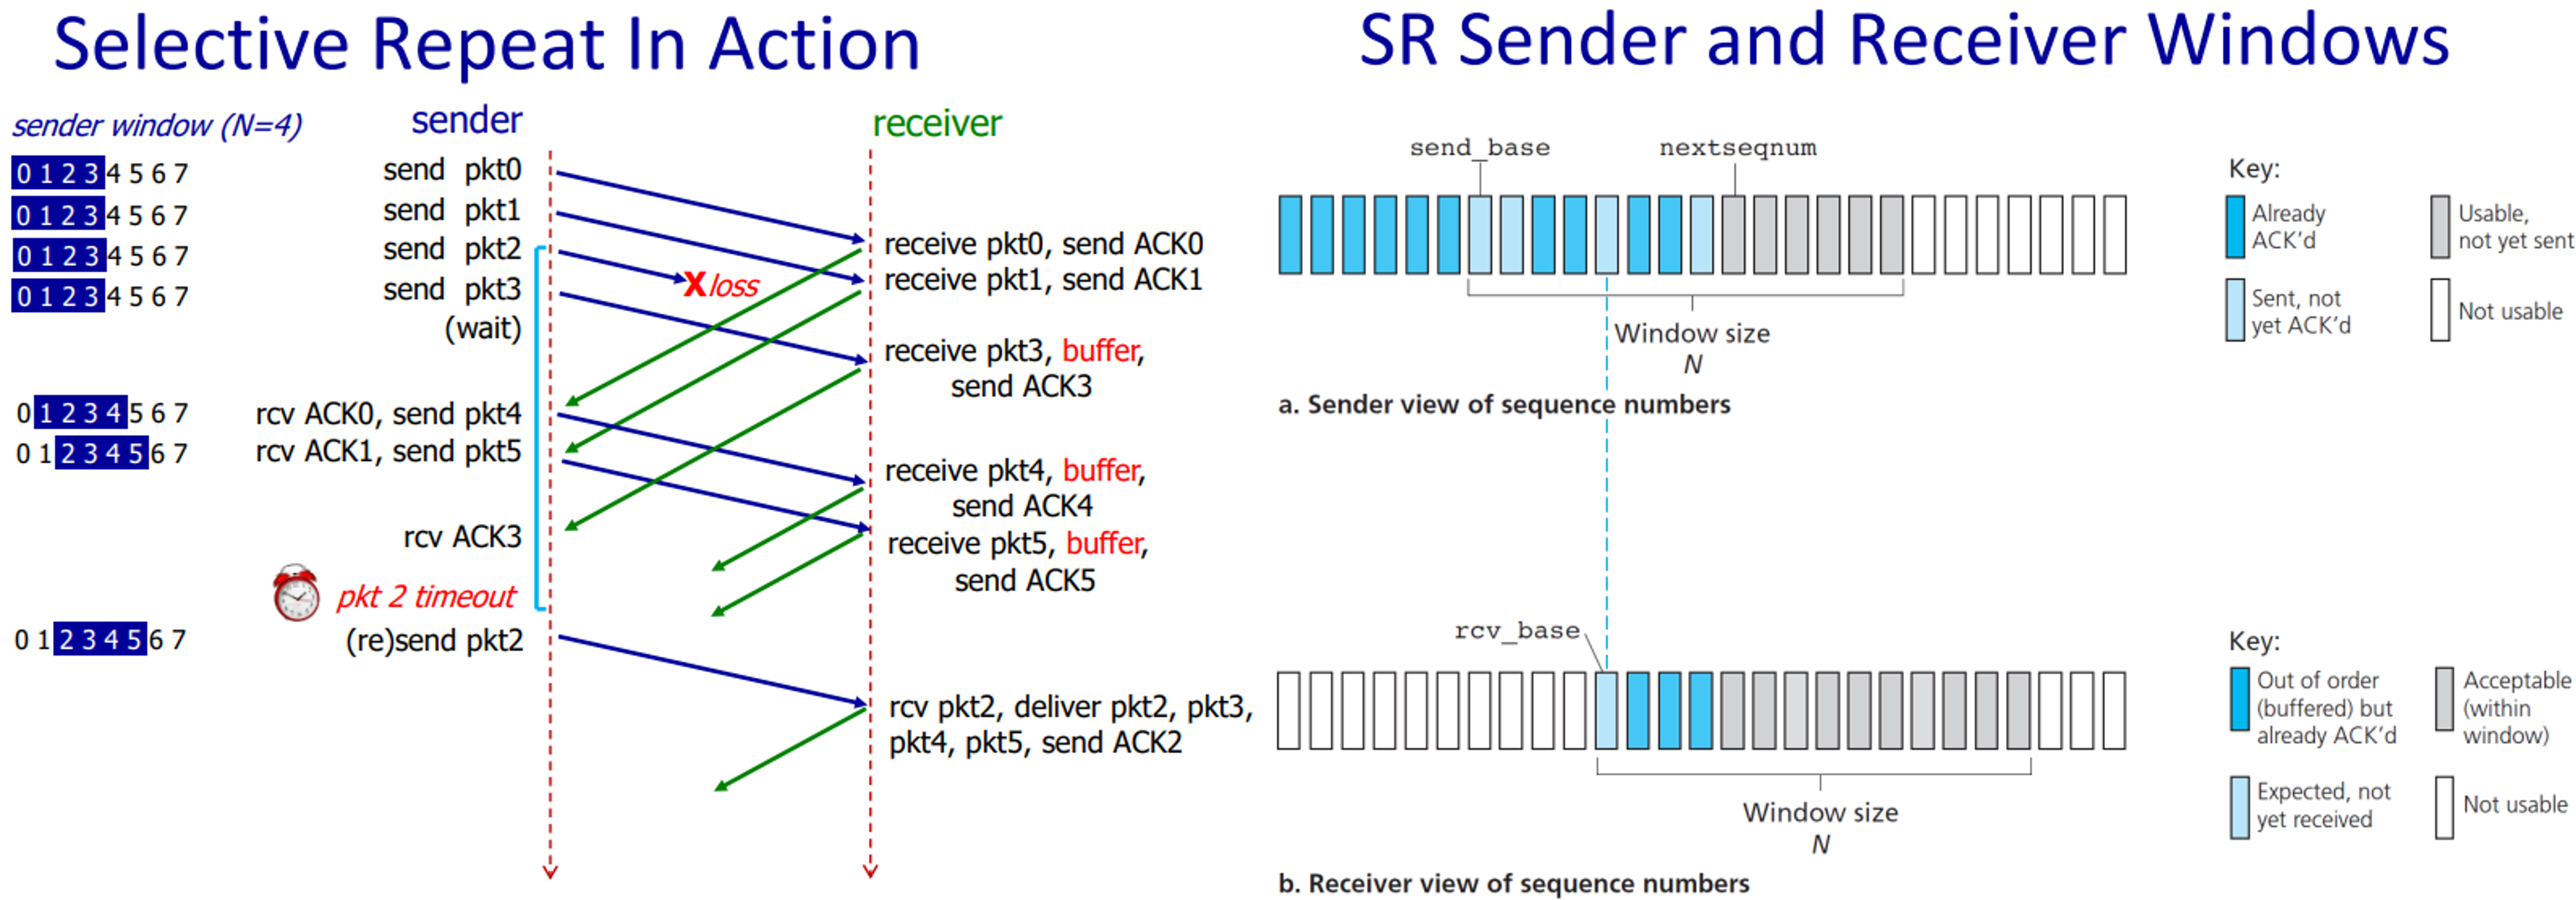
\includegraphics[width=1\linewidth]{selectiver}}



\section{TCP: Connection-oriented Transport}
\begin{itemize}
\item \textbf{Connection oriented}: handshake before sending data. \textbf{Point to point}: one sender, one receiver. The connection is \textbf{duplex} (bidirectional data flow). \textbf{Reliable in-order}.
\item TCP socket is fully identified by four-tuple: (source IP addr, source port no., dest IP addr, dest port no.). 
\item \textbf{Multiplexing}: TCP gathers data from processes, form transport-layer segments including app data and 4-tuple pass to network layer. 
\item \textbf{Demultiplexing}: Connection socket created, server already noted 4-tuple. Subsequent packets directed, or demultiplexed, to the appropriate socket using those 4 values.
\item TCP creates \textbf{buffers} after handshaking. 
\end{itemize}

\subsubsection{TCP Segment / Header}
\begin{itemize}
\item The maximum segment size (MSS) depends on maximum transmission unit (MTU). 
\item Generally MSS is 1460 bytes, (MTU is 1500 bytes for Ethernet and PPP link-layer protocols.) 40 bytes split half for TCP and IP header.
\item TCP Seq. no is "byte no.", first b of data in segment.
\item TCP Ack. no is "seq no." of next b expected by receiver.
\item Checksum computation uses 1s complement (UDP same)
\smallskip
\centerline{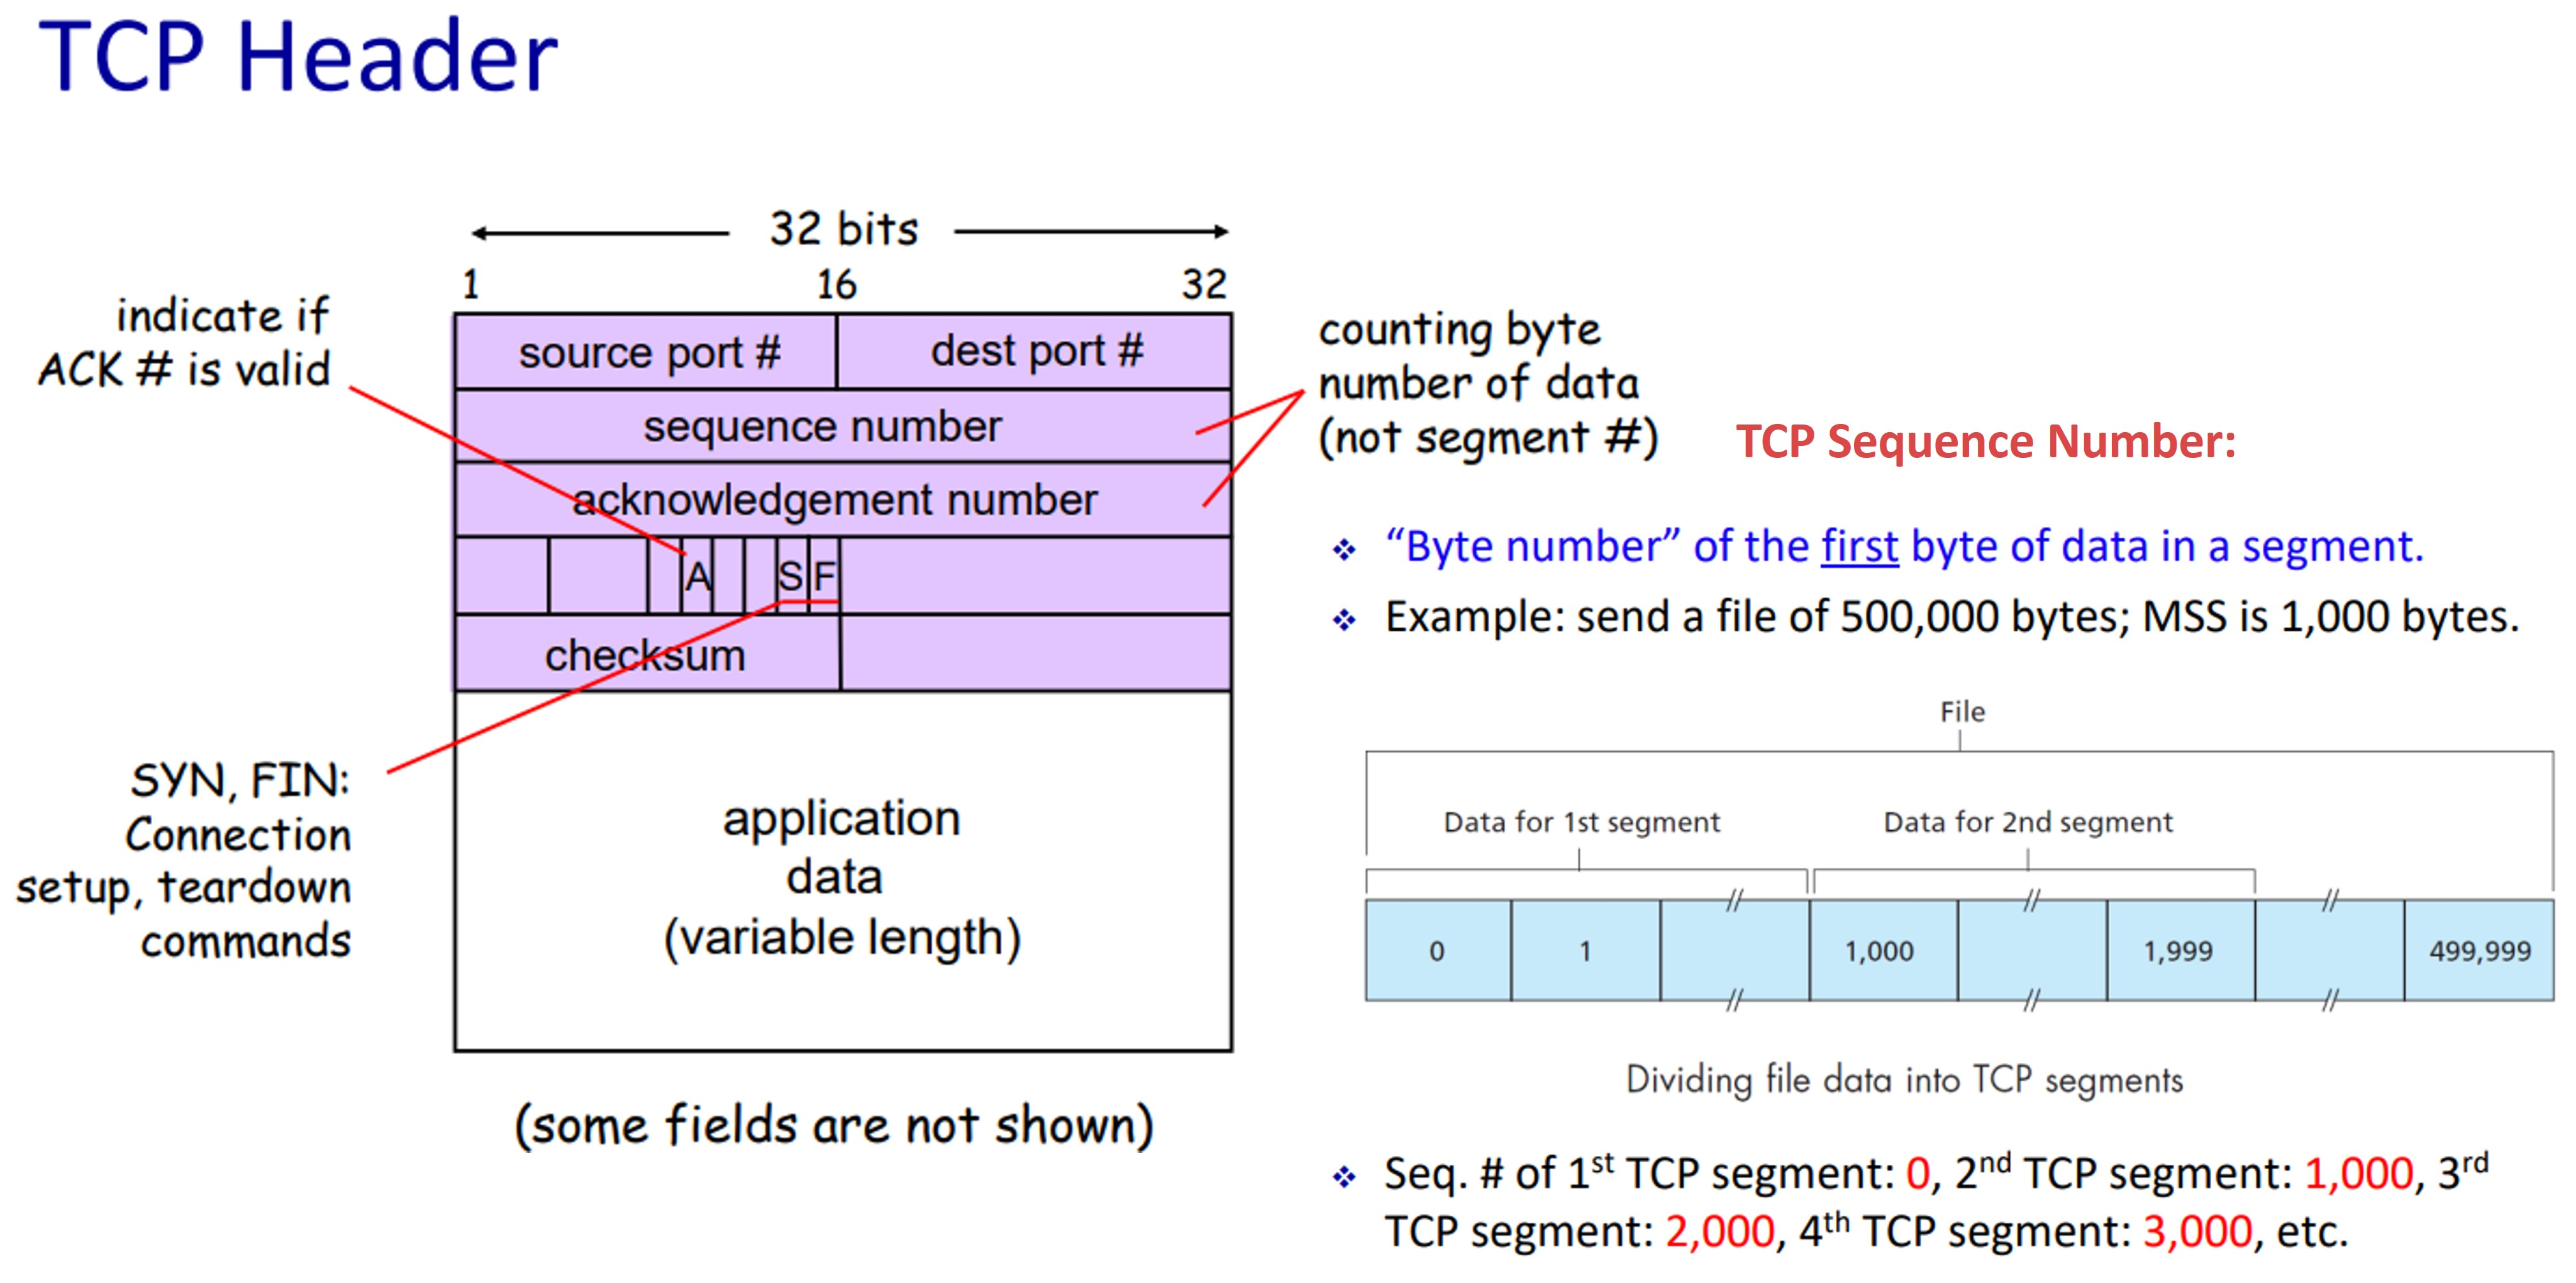
\includegraphics[width=1\linewidth]{tcpheader}}
\medskip
\centerline{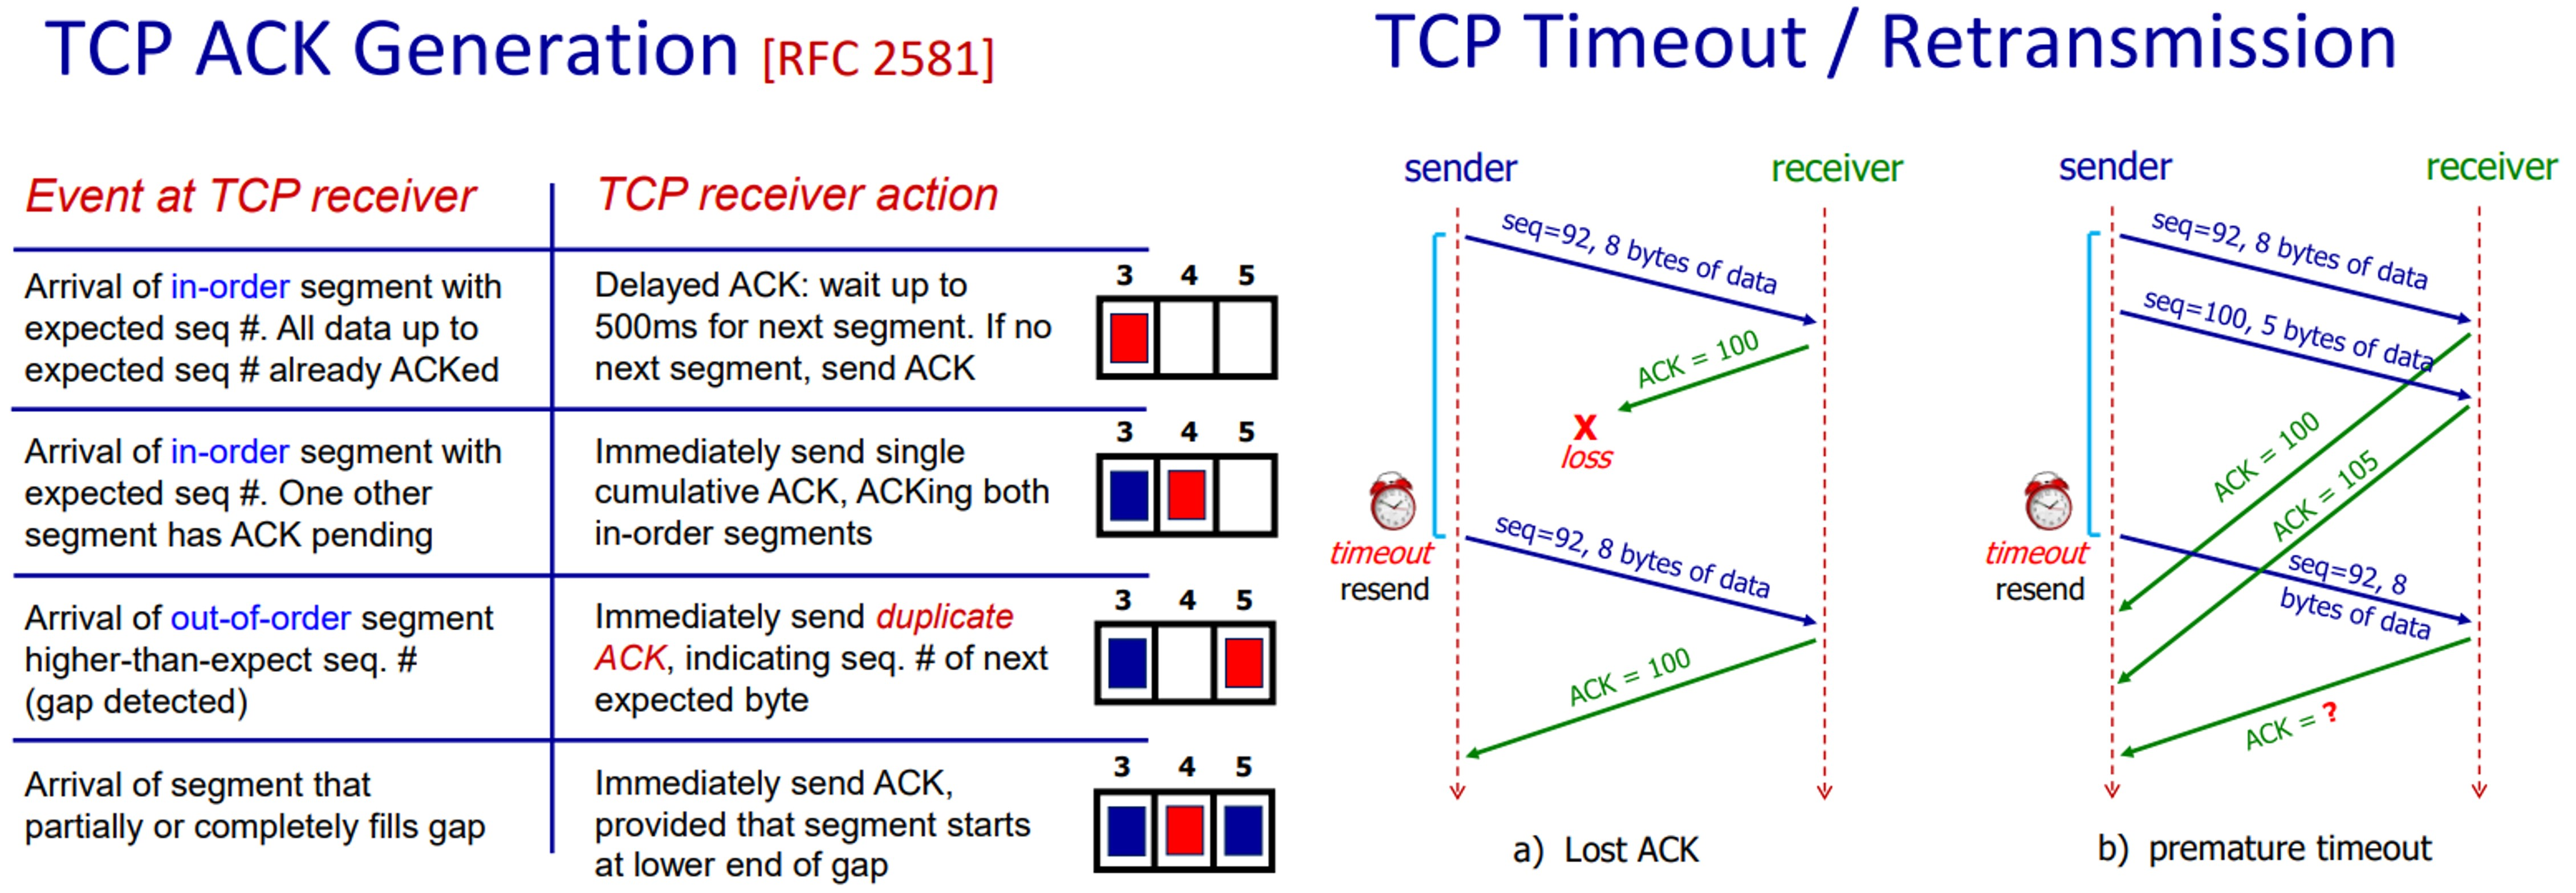
\includegraphics[width=1\linewidth]{TCPACKgen}}
\item Random initial sequence number: Minimise probability of some segment from previous connection mistaken as from current connection
\end{itemize}

% \vfill \null
% \columnbreak

\subsubsection{TCP Timeout Value}
\begin{itemize}
\item Determining TCP appropriate timeout value:
\item too short timeout: premature timeout and unnecessary retransmissions.
\item too long timeout: slow reaction to segment loss. Timeout interval must be longer than RTT – but RTT varies!
\item TCP computes (and keeps updating) timeout interval based on estimated RTT. (TimeoutInterval = EstimatedRTT + 4*DevRTT)
\end{itemize}

\subsubsection{TCP Fast Retransmission}
\begin{itemize}
\item Timeout period is often relatively long. long delay before resending lost packet.
\item \textbf{Fast retransmission}: If sender receives 4 ACKs for same segment, suppose segment is lost, resend segment (even before timer expires).
\end{itemize}
\smallskip
\centerline{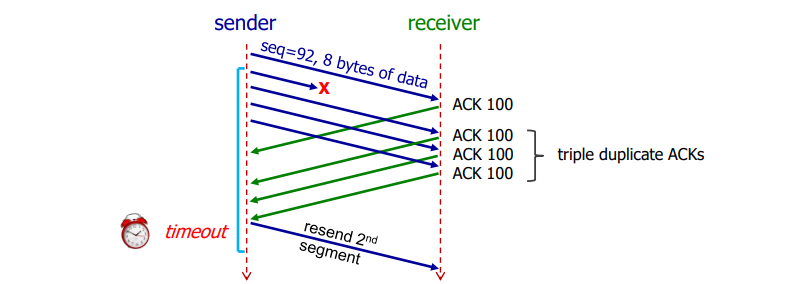
\includegraphics[width=1\linewidth]{fastretransmit}}
\smallskip

\subsubsection{TCP Handshake / Closing}
\begin{itemize}
\item Before exchanging app data, TCP sender and receiver “shake hands”, agree on connection and exchange connection parameters.
\item Closing: Client, server each close their side of connection, send TCP segment with FIN bit = 1 
\end{itemize}
\smallskip
\centerline{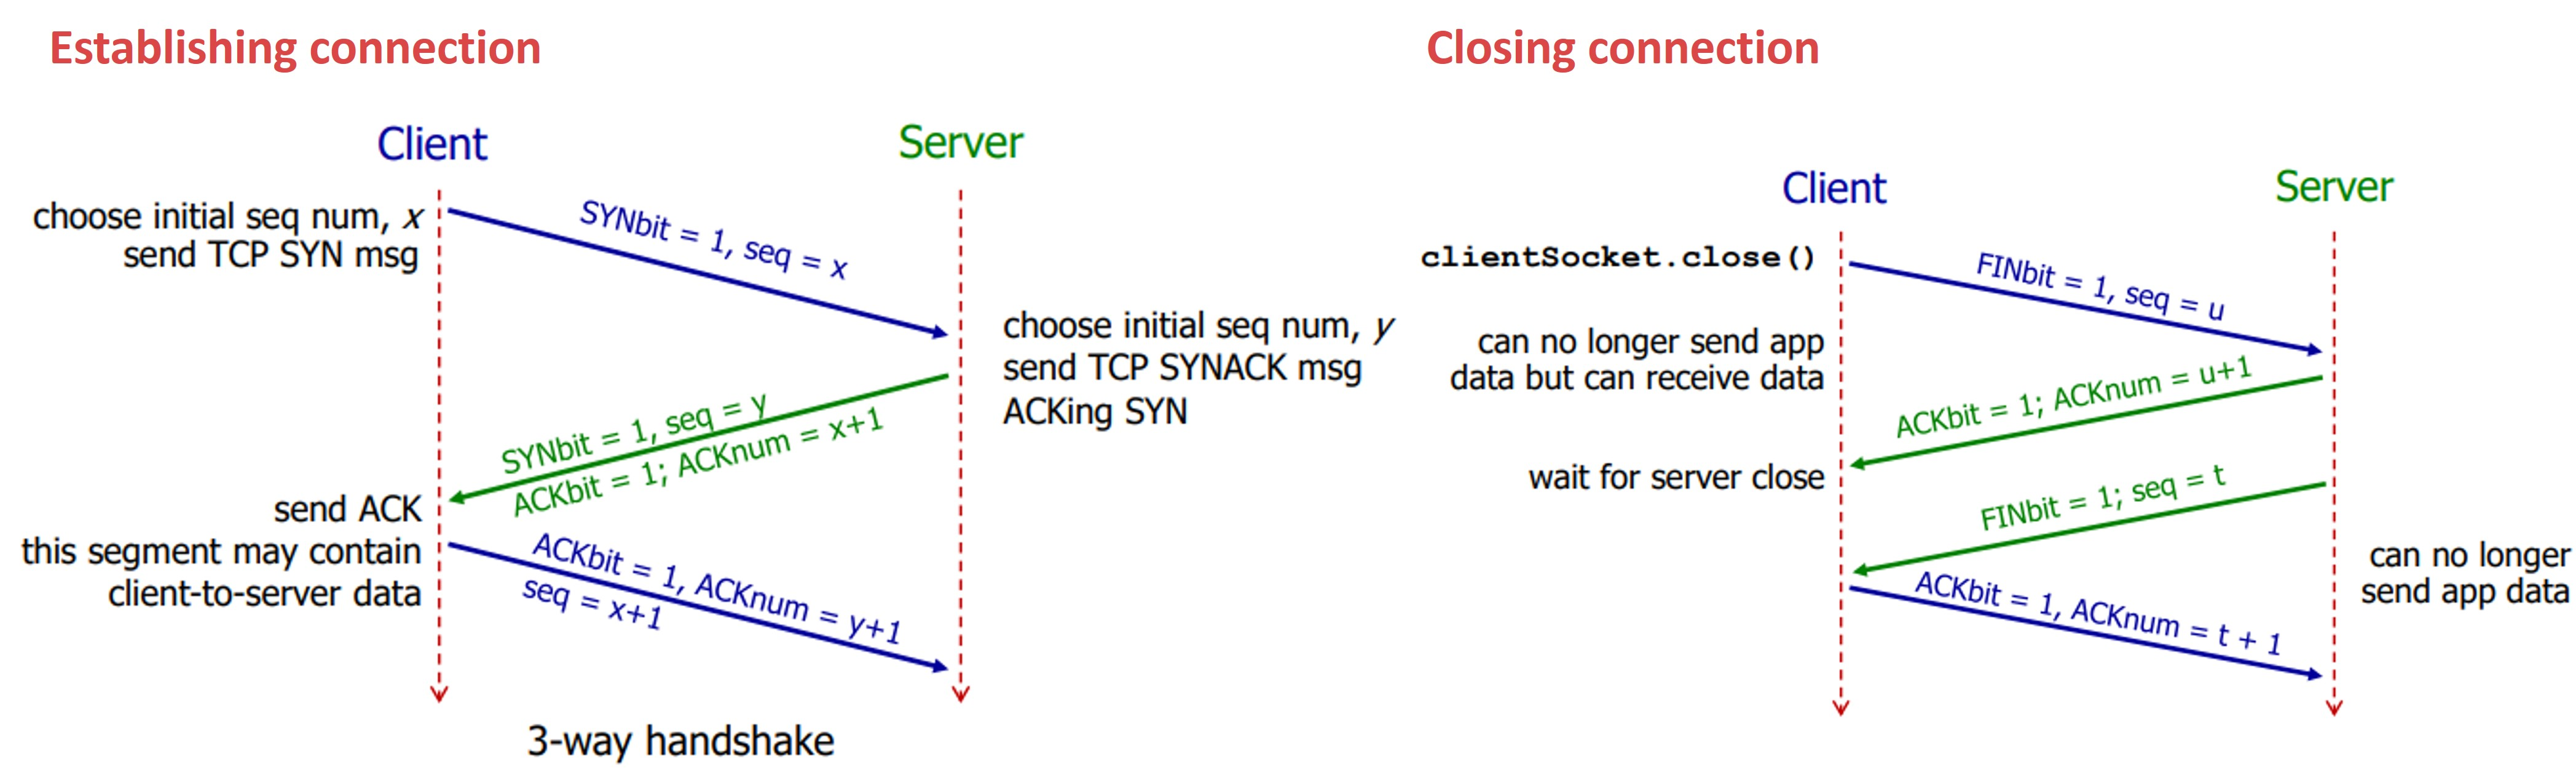
\includegraphics[width=1\linewidth]{tcpconnection}}

% \vfill \null
% \columnbreak

\section{4. Network}
\subsubsection{Network Layer Services}
\begin{itemize}
\item Network layer delivers packets to receiving hosts.
\item Routers examine header fields of IP datagrams passing it.
\item \textbf{Forwarding}: Moving of incoming packet to appropriate output link.
\item \textbf{Routing}: Calculation of path taken by packets from sender to receiver.


\end{itemize}

\subsubsection{IP Address}
\begin{itemize}
\item \textbf{IP address} used to identify host / (router), 32-bit integer expressed in binary/decimal.
\item Host gets an IP address either through manual configuration by sys admin, or auto assigned by a \textbf{DHCP} server.
\end{itemize}

\centerline{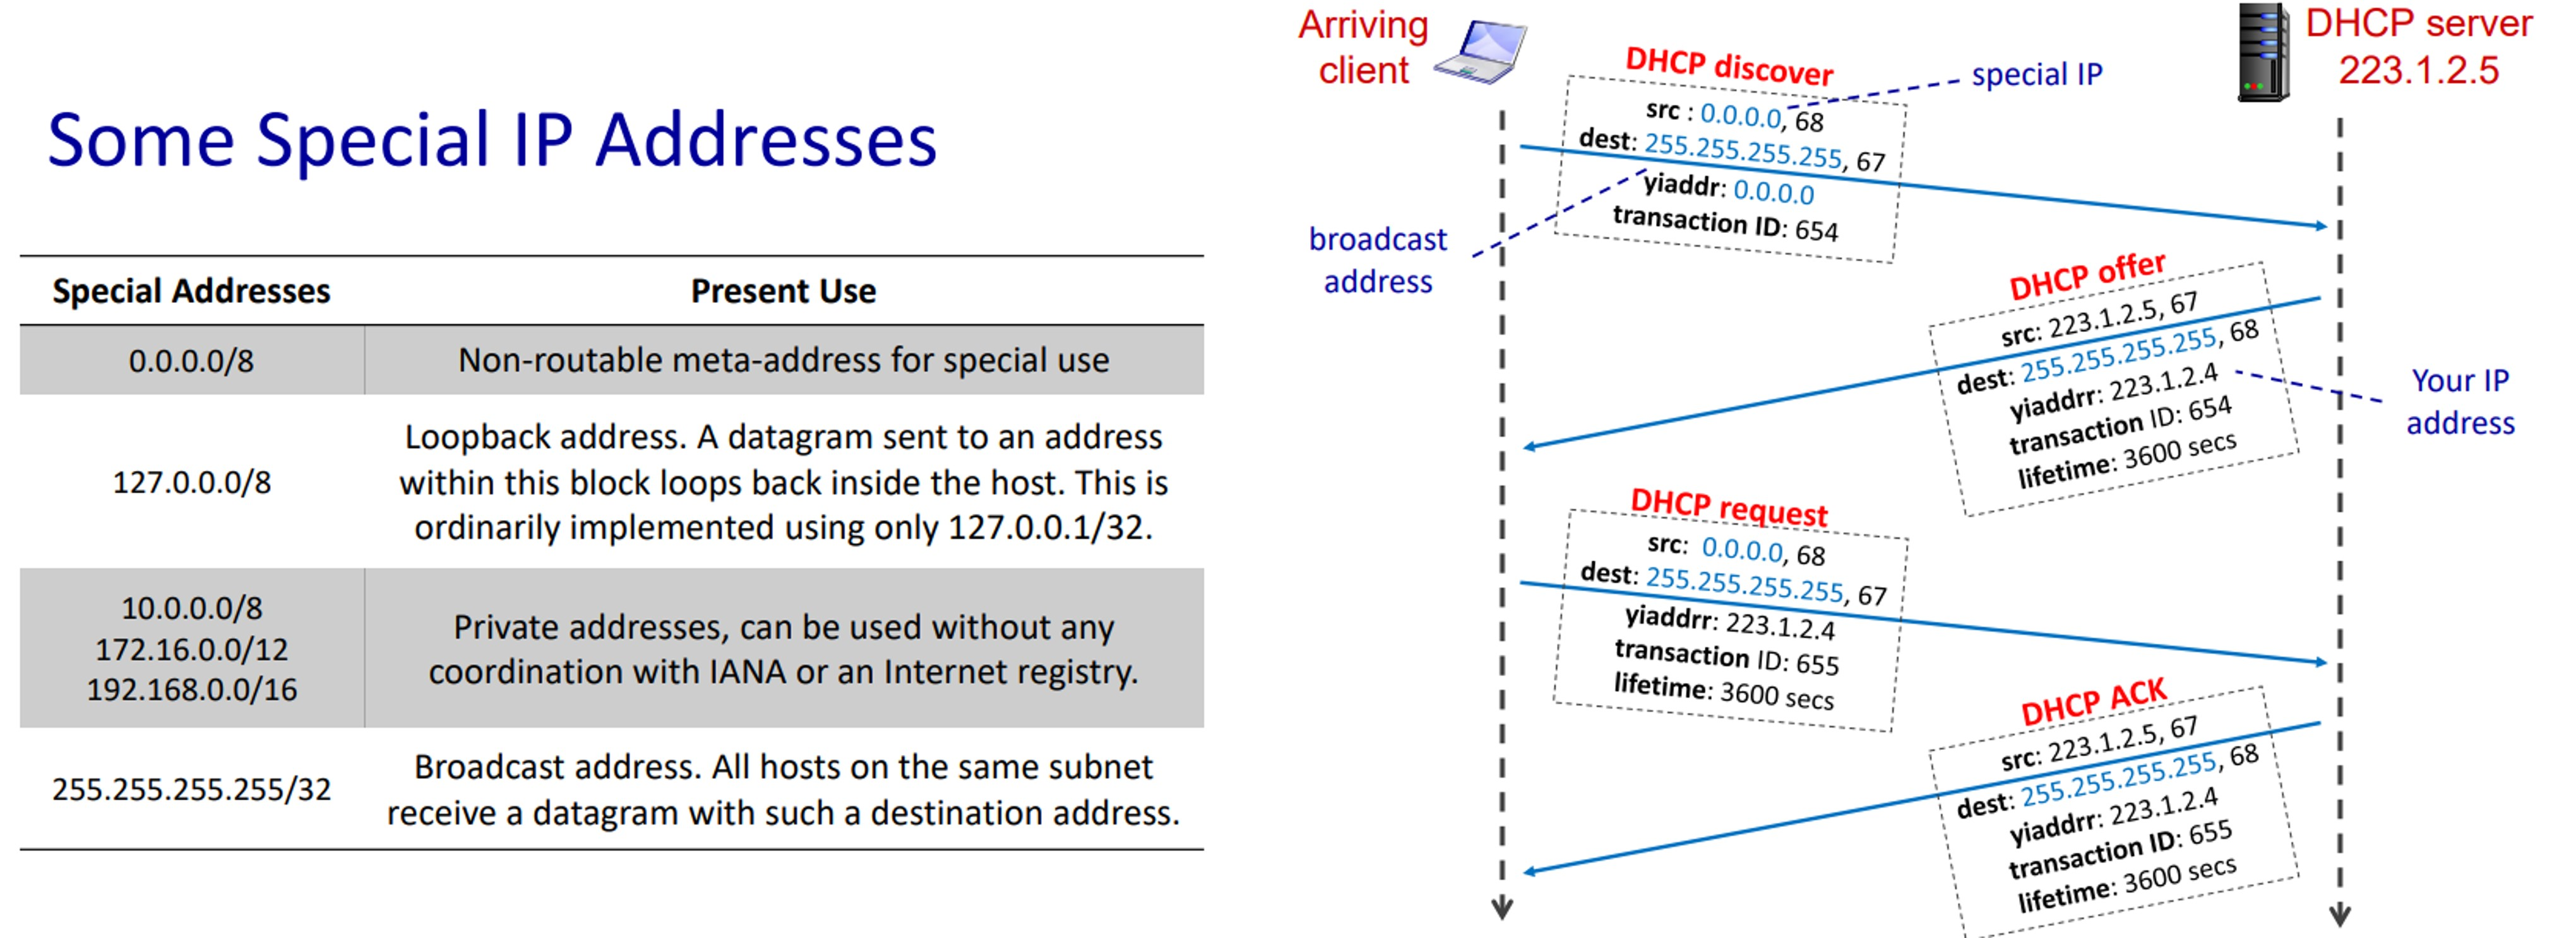
\includegraphics[width=1\linewidth]{dhcp}}

\subsubsection{DHCP: Dynamic Host Configuration Protocol}
\begin{itemize}
\item \textbf{DHCP} allows a host to dynamically obtain its IP address from DHCP server when it joins network.
\item IP address is \underline{renewable}, allow \underline{reuse} of addresses (only hold address while connected), support mobile users to join network.
\item DHCP: 4-step process: Host broadcasts “DHCP discover” message, server responds with “DHCP offer” message, Host requests IP address: “DHCP request” message, DHCP server sends address: “DHCP ACK” message
\item  DHCP may provide host additional network information, e.g. IP of first-hop router, local DNS server, network mask.
\item DHCP runs over \textbf{UDP}. DHCP server port 67, client port 68.
\end{itemize}

\subsubsection{IP Address \& Network Interface}
\begin{itemize}
\item IP address is associated with a network interface.
\item Host usually has one or two network interfaces (e.g. wired Ethernet and WiFi), A router typically has  multiple interfaces.
\item \textbf{IP Addr} comprises network/subnet prefix and host ID.
\end{itemize}

\subsubsection{Subnet}
\begin{itemize}
\item \textbf{Subnet} is a network formed by a group of “directly” interconnected hosts.
\item Hosts in same subnet have same network prefix of IP addr, can physically reach each other without intervening router. They connect to the outside world through a router
\item \textbf{Classless Inter-domain Routing} (CIDR): Internet’s IP address assignment strategy.
\item Subnet prefix of IP addr of arbitrary length, Address format: $a.b.c.d/x$, where $x$ is the no. of bits in subnet prefix of IP addr.
\item \textbf{Subnet mask} is used to determine which subnet an IP address belongs to.
\item made by setting all subnet prefix bits to "1"s and host ID bits to "0"s.
\end{itemize}

\medskip
\centerline{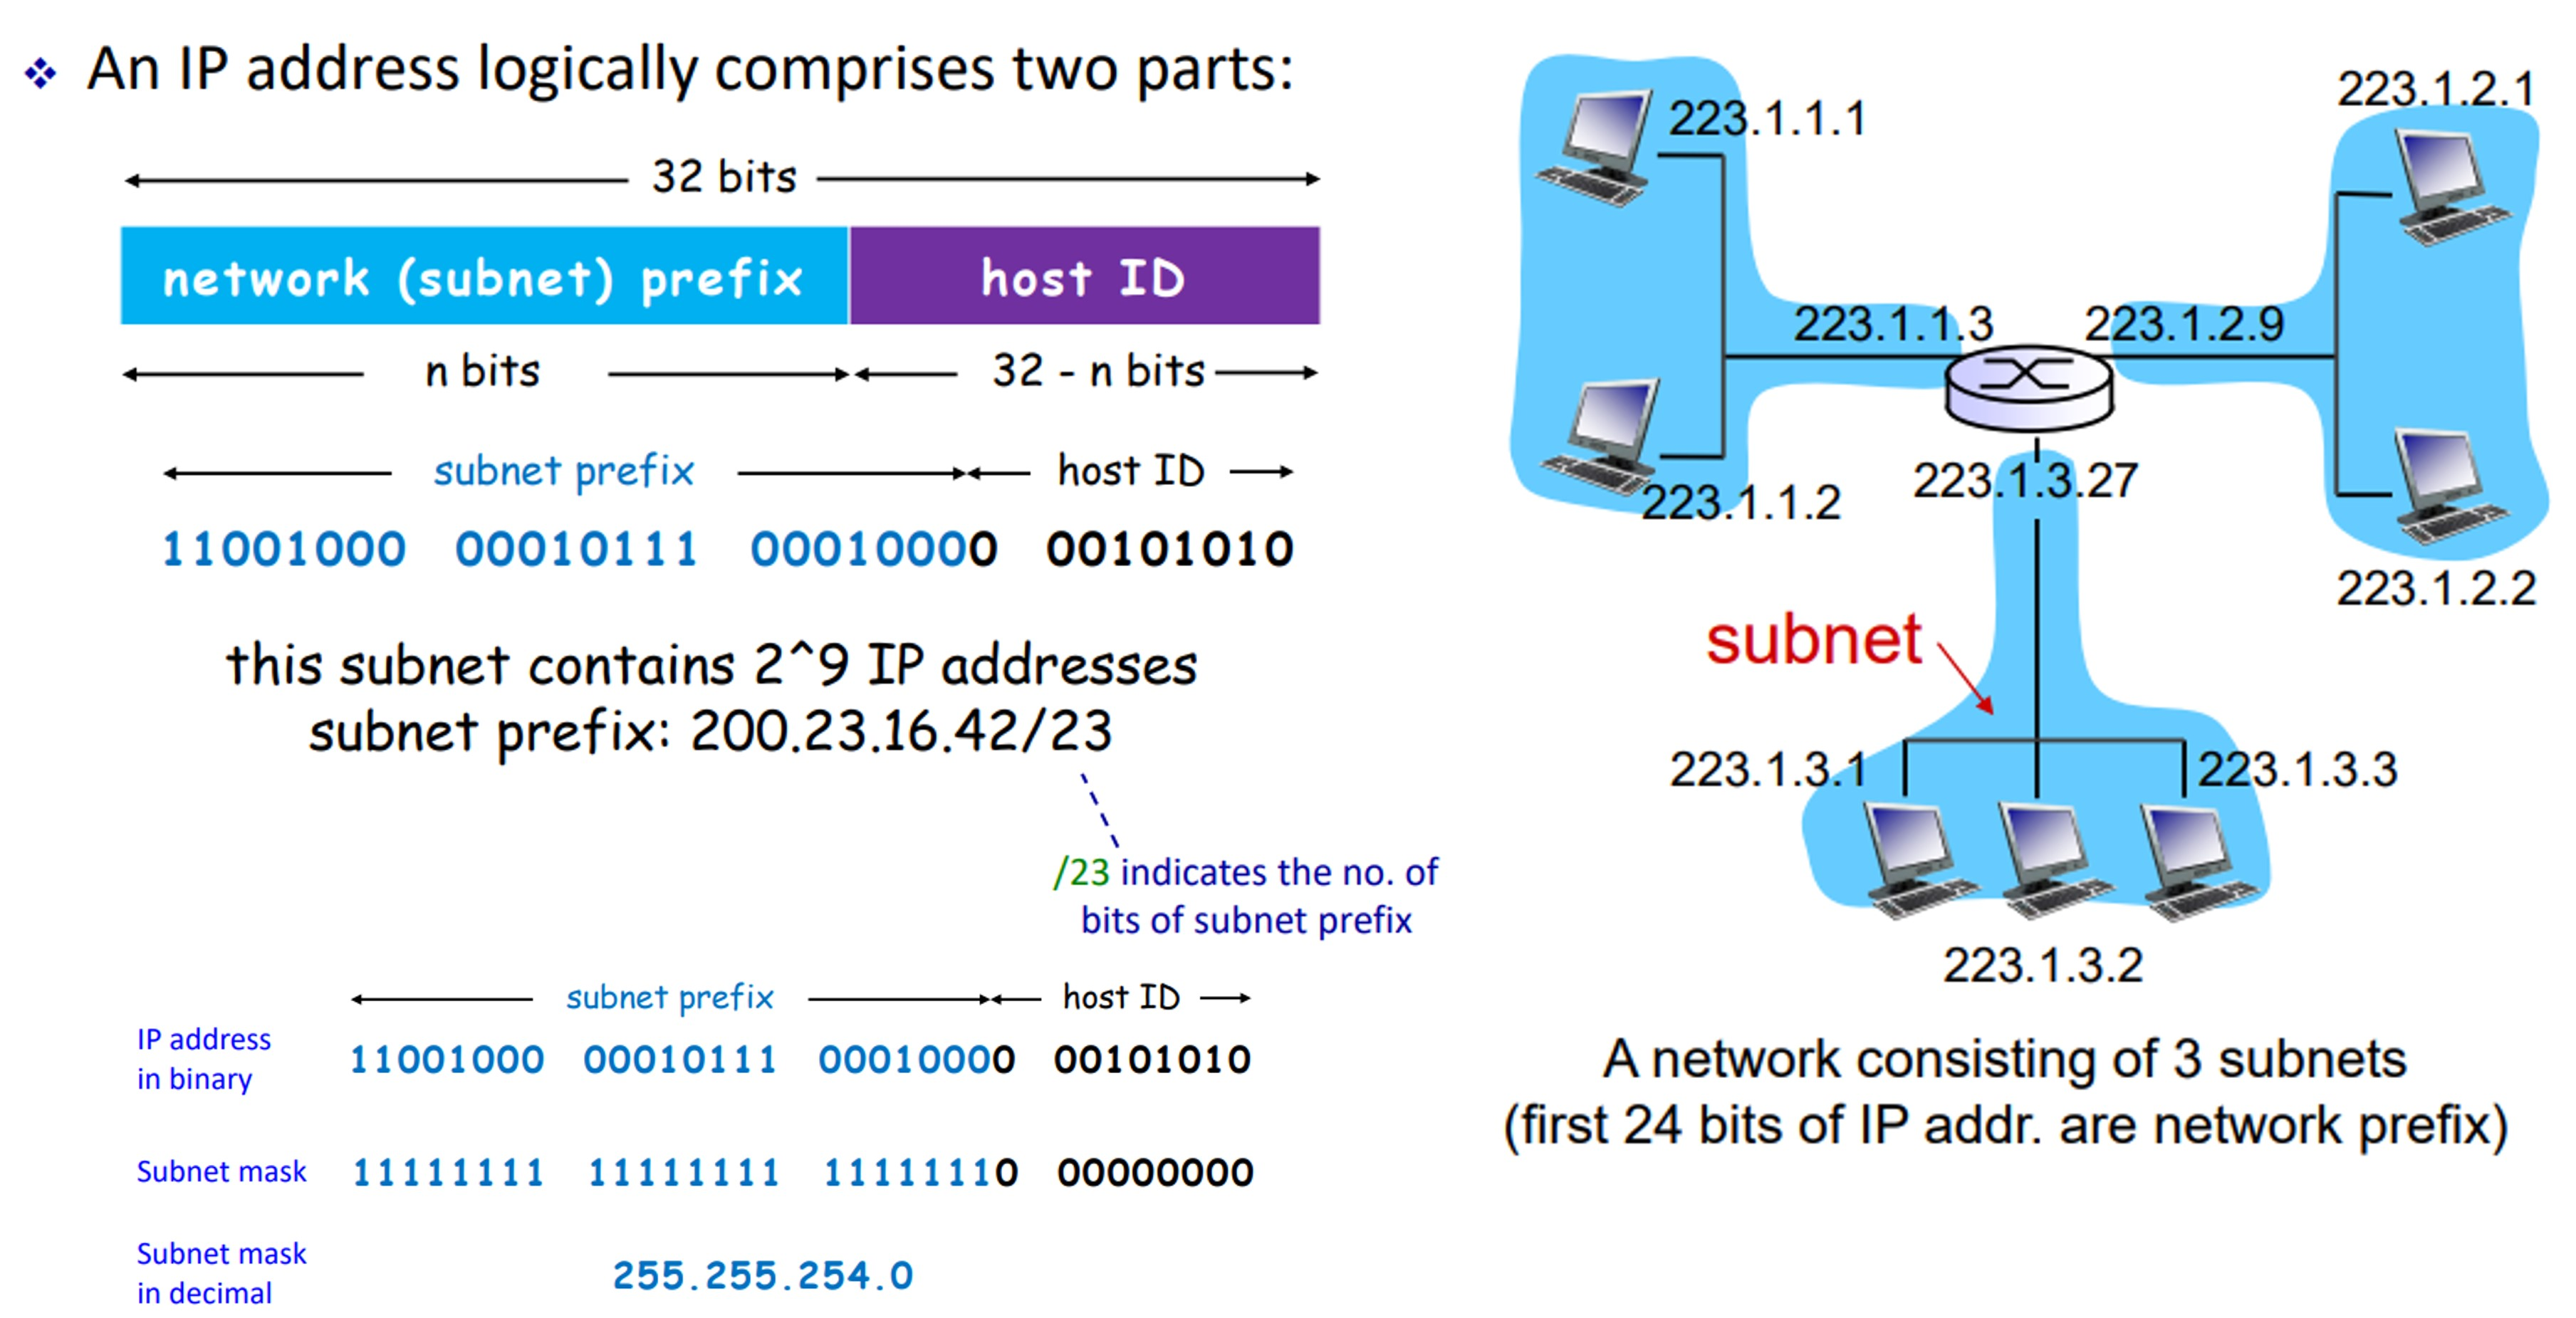
\includegraphics[width=1\linewidth]{ipsubnet}}

\vfill \null

\subsubsection{IP Address Allocation}
\begin{itemize}
\item Organization can buy from registry / rent from ISP’s addr space to obtain block of IP addr.
\item \textbf{Hierarchical Addressing}: Allows efficient way of routing.
\centerline{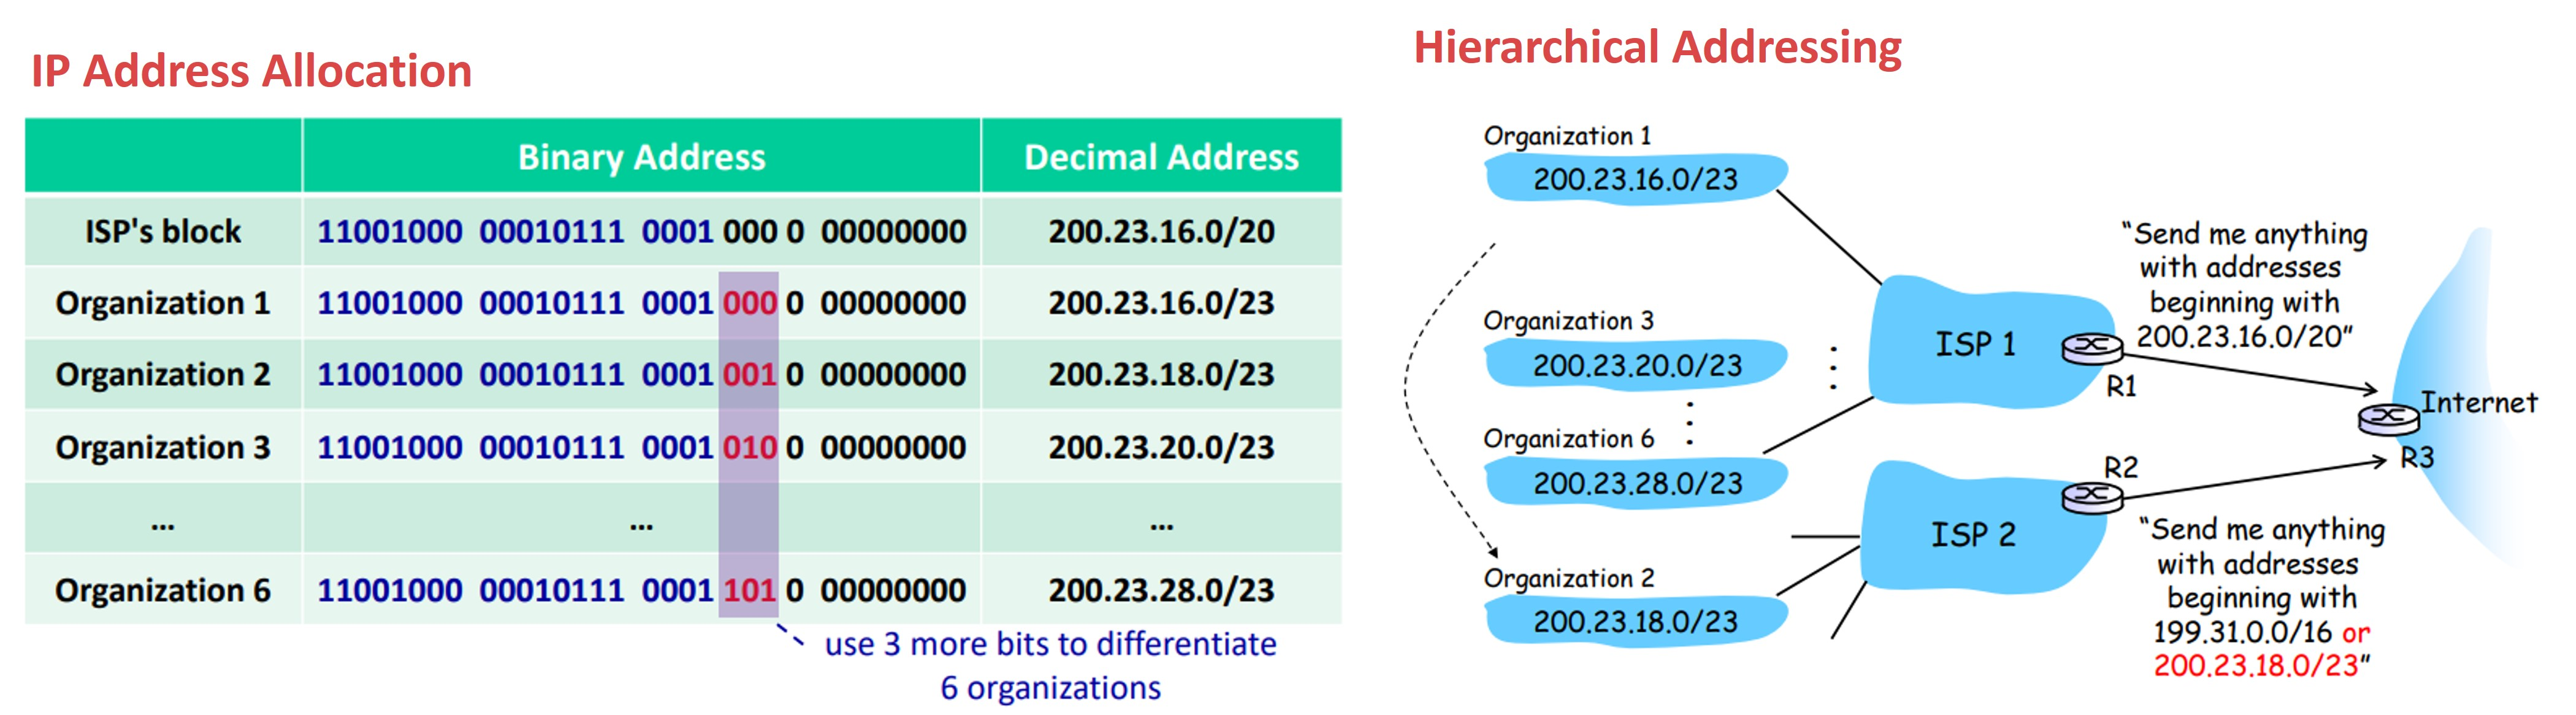
\includegraphics[width=1\linewidth]{IPaddressHA}}
\item \textbf{Longest Prefix Match}: Choose one with longer match. If IP addrr matches all 23 bits for org, packet forwarded, else forwarded to latter.
\end{itemize}

\subsubsection{Network Address Translation (NAT)}
\begin{itemize}
\item Map IP addr space by modifying network addr info in packets IP header through traffic routing device. NAT Routers must:
\item \textbf{Replace} \underline{(source IP address, port \#)} of every outgoing datagram to \underline{(NAT IP address, new port \#)}, \textbf{Remember} (in NAT translation table) the mapping and \textbf{Replace} destination fields of every incoming datagram with that stored in NAT translation table.
\item \textbf{Benefits}: Single public IP for NAT router allows multiple private IP address. Change (private IP) addr of hosts in local network without notifying outside world.
\item ISP change w/o changing local host addresses in local network.
\item Hosts inside local network not explicitly addressable or visible by outside world (security plus).
\medskip
\centerline{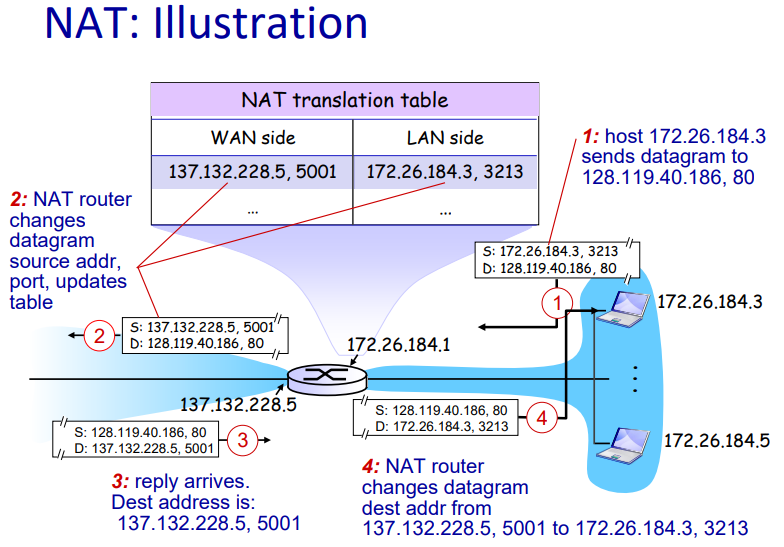
\includegraphics[width=0.85\linewidth]{nat}}
\end{itemize}

\subsubsection{Routing Algorithms}
\begin{itemize}
\item The Internet as \textbf{“network-of-networks”}, hierarchy of \textbf{Autonomous Systems} (AS), e.g., ISPs, each owns routers and links.
\item Due to size and decentralized administration of Internet, routing is done hierarchically.
\item \textbf{Intra-AS routing}: Finds good path btwn two routers within AS. Commonly used protocols: RIP, OSPF
\item \textbf{Inter-AS routing (not covered)} Handles the interfaces between ASs, standard protocol: BGP.
\end{itemize}


\subsubsection{Intra-AS Routing}
\begin{itemize}
\item Abstractly view a network of routers as a graph, vertices are routers, edges are physical links between routers.
\item Associate cost to each link. (cost = 1, or inversely related to bandwidth, or related to congestion)
\item \textbf{Routing}: find least cost path btwn two vertices in graph.
\item \textbf{Link state Algorithmns}: Centralised routing algo, all routers have complete knowledge of network topology and link costs. Routers periodically broadcast link costs to each other.
\item Use Dijkstra algorithm compute least cost path locally! (using global map).
\item \textbf{Distance vector Algorithms}: Decentralised routing algo, Routers know physically-connected neighbors and link costs to neighbors.
\item Routers exchange “local views” with neighbors, update own “local views”. Iterative computation: Swap local view with direct neighbours, Update own view, Repeat till no further change. 
\end{itemize}

\subsubsection{Distance Vector Algo (Bellman Ford)}
\begin{itemize}
\centerline{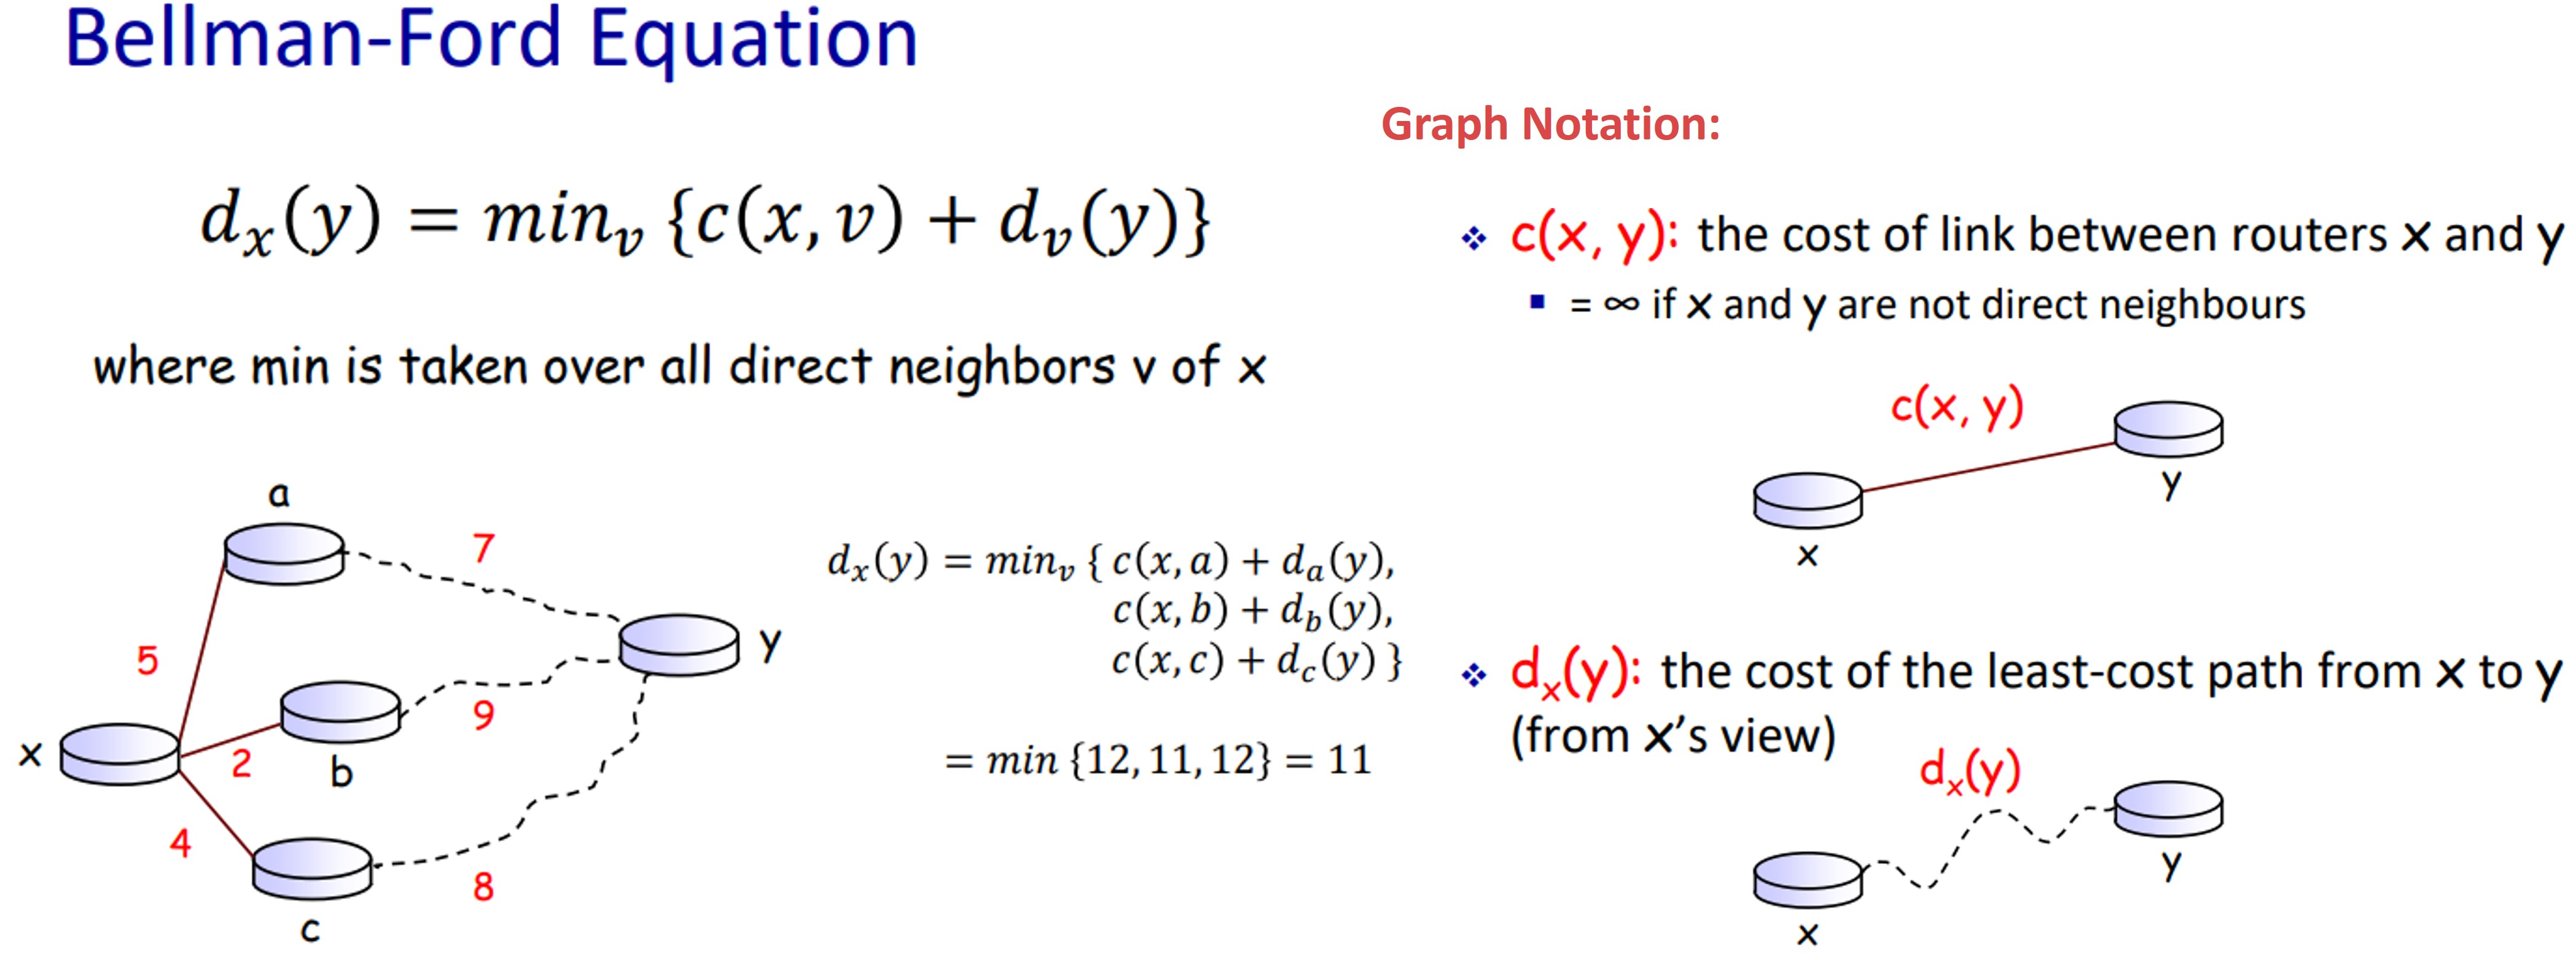
\includegraphics[width=1\linewidth]{bmf}}
\bigskip
\item \textbf{$d_x(y) = min_v \{c(x,v) + d_v(y)\}$}
\item To find \textbf{least cost path}, x needs to know cost from each of its direct neighbour to y. Each neighbour v sends its distance vector (y, k) to x, telling x that the cost from v to y is k.
\item Every router, x, y, z, sends its distance vectors to directly connected neighbors. When x finds y is advertising cheaper path to z than known, x update distance vector to z accordingly and note down all packets for z should be sent to y. Info used to create forwarding table of x.
\item After every router exchanged several rounds of updates with direct neighbors, all routers will know least-cost paths to all other routers.
\end{itemize}

\subsubsection{RIP (Routing Information Protocol)}
\begin{itemize}
\item \textbf{RIP} implements the DV algorithm. Uses hop count as the cost metric (insensitive to network congestion).
\item Exchange routing table every 30 seconds over UDP port 520.
\item “Self-repair”: if no update from a neighbour router for 3 minutes, assume neighbour failed.
\end{itemize}


\subsubsection{Internet Protocol (IP): IPv4}
\begin{itemize}
\medskip
\centerline{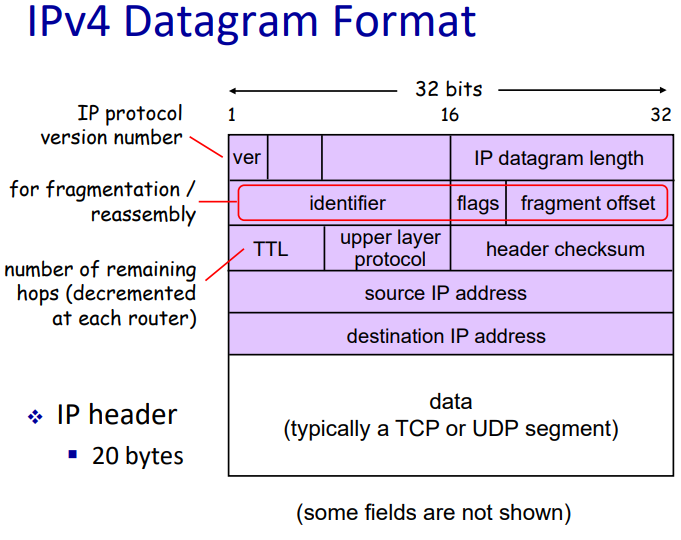
\includegraphics[width=0.9\linewidth]{ipv4datagram}}
\item Length: of IP datagram + 20b header. Identifier, flags, fragment offset: support fragmentation \& reassembly
\item TTL: Prevent infinite circulation. Upper layer protocol: Only used at final dest, determine if UDP/TCP (for Internet). Checksum also uses 1s complement.
\item \textbf{IPv6}: 40b header with 128b IP addr.
\end{itemize}

\subsubsection{IP Fragmentation \& Reassembly}
\begin{itemize}
\item Different links, different MTU (Max Transfer Unit, max amt of data link-level frame can carry).
\item “Too large” IP datagrams may be fragmented by routers. \\
\centerline{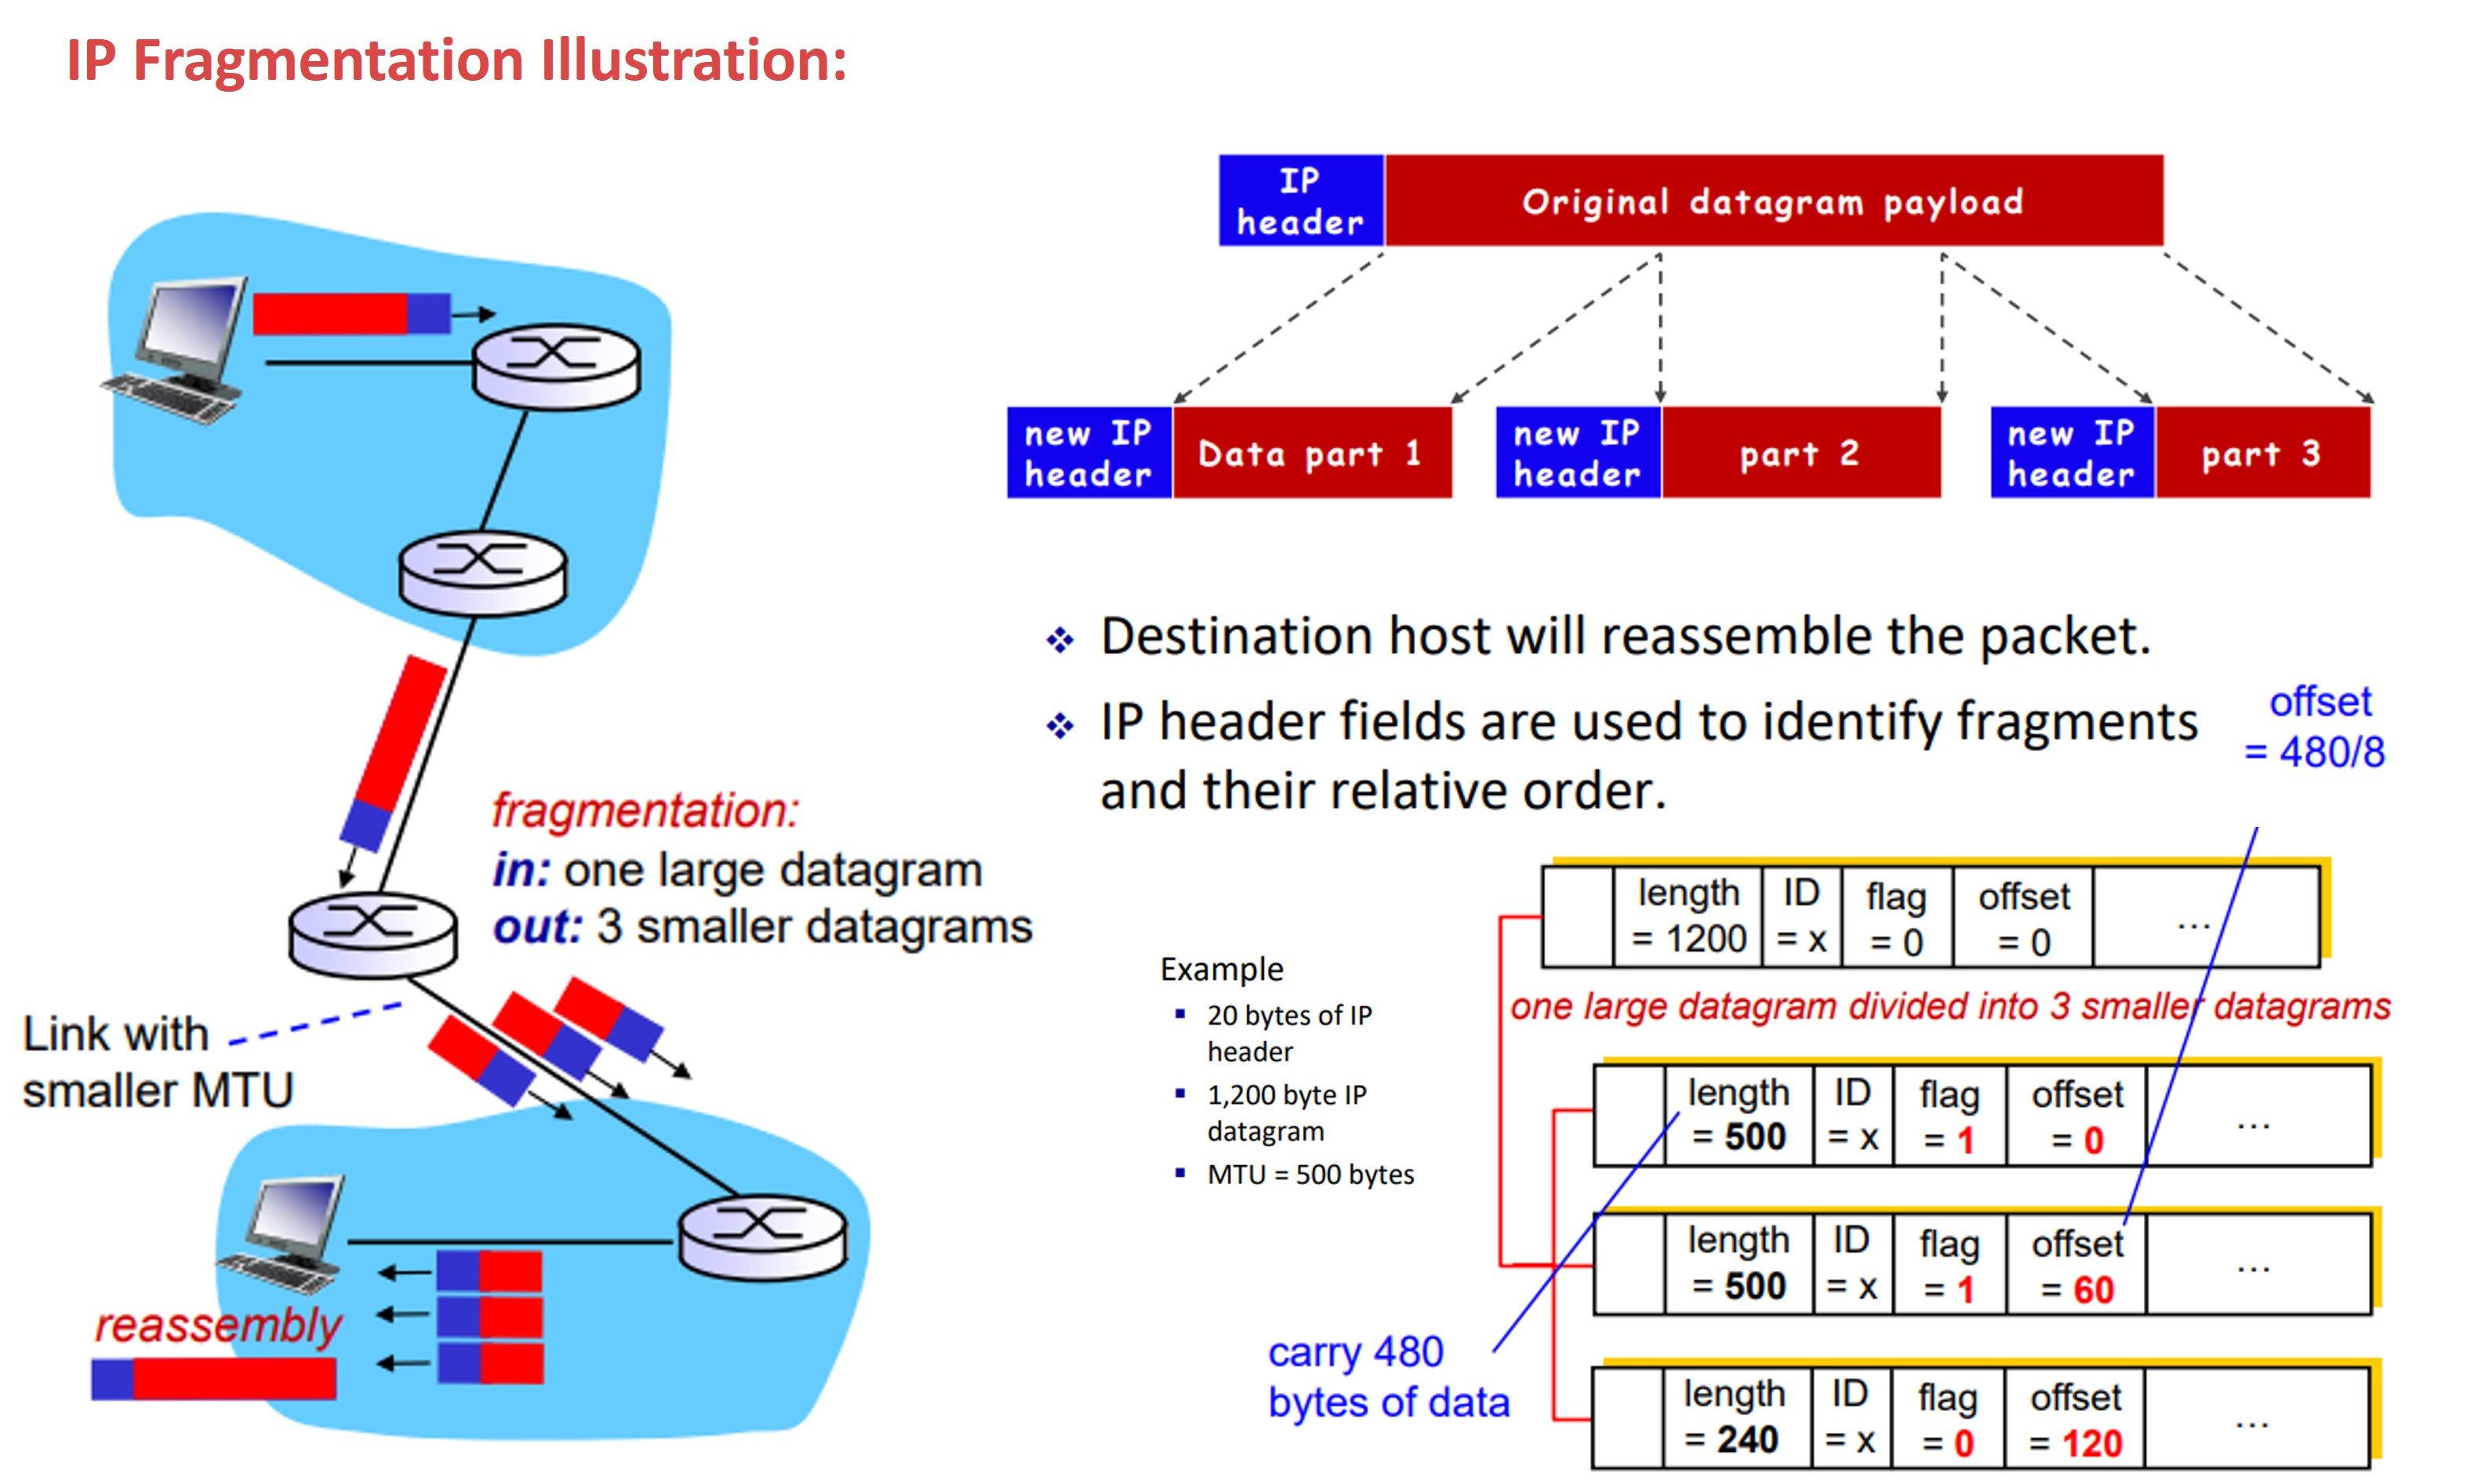
\includegraphics[width=0.9\linewidth]{ipfragmentation}}
\medskip
\item \textbf{Flag}(frag flag) is set to 1 if next fragment from same segment, 0 if this is the last fragment.
\item \textbf{Offset} is in expressed in unit of 8-bytes
\end{itemize}

\subsubsection{Internet Control Message Protocol}
\begin{itemize}
\item \textbf{ICMP}: used by hosts \& routers to communicate network-level information.
\item \textbf{Error reporting}: unreachable host / network / port / protocol.
\item Echo request/reply (used by ping).
\item ICMP messages carried in IP datagrams, ICMP header starts after IP header.
\medskip
\centerline{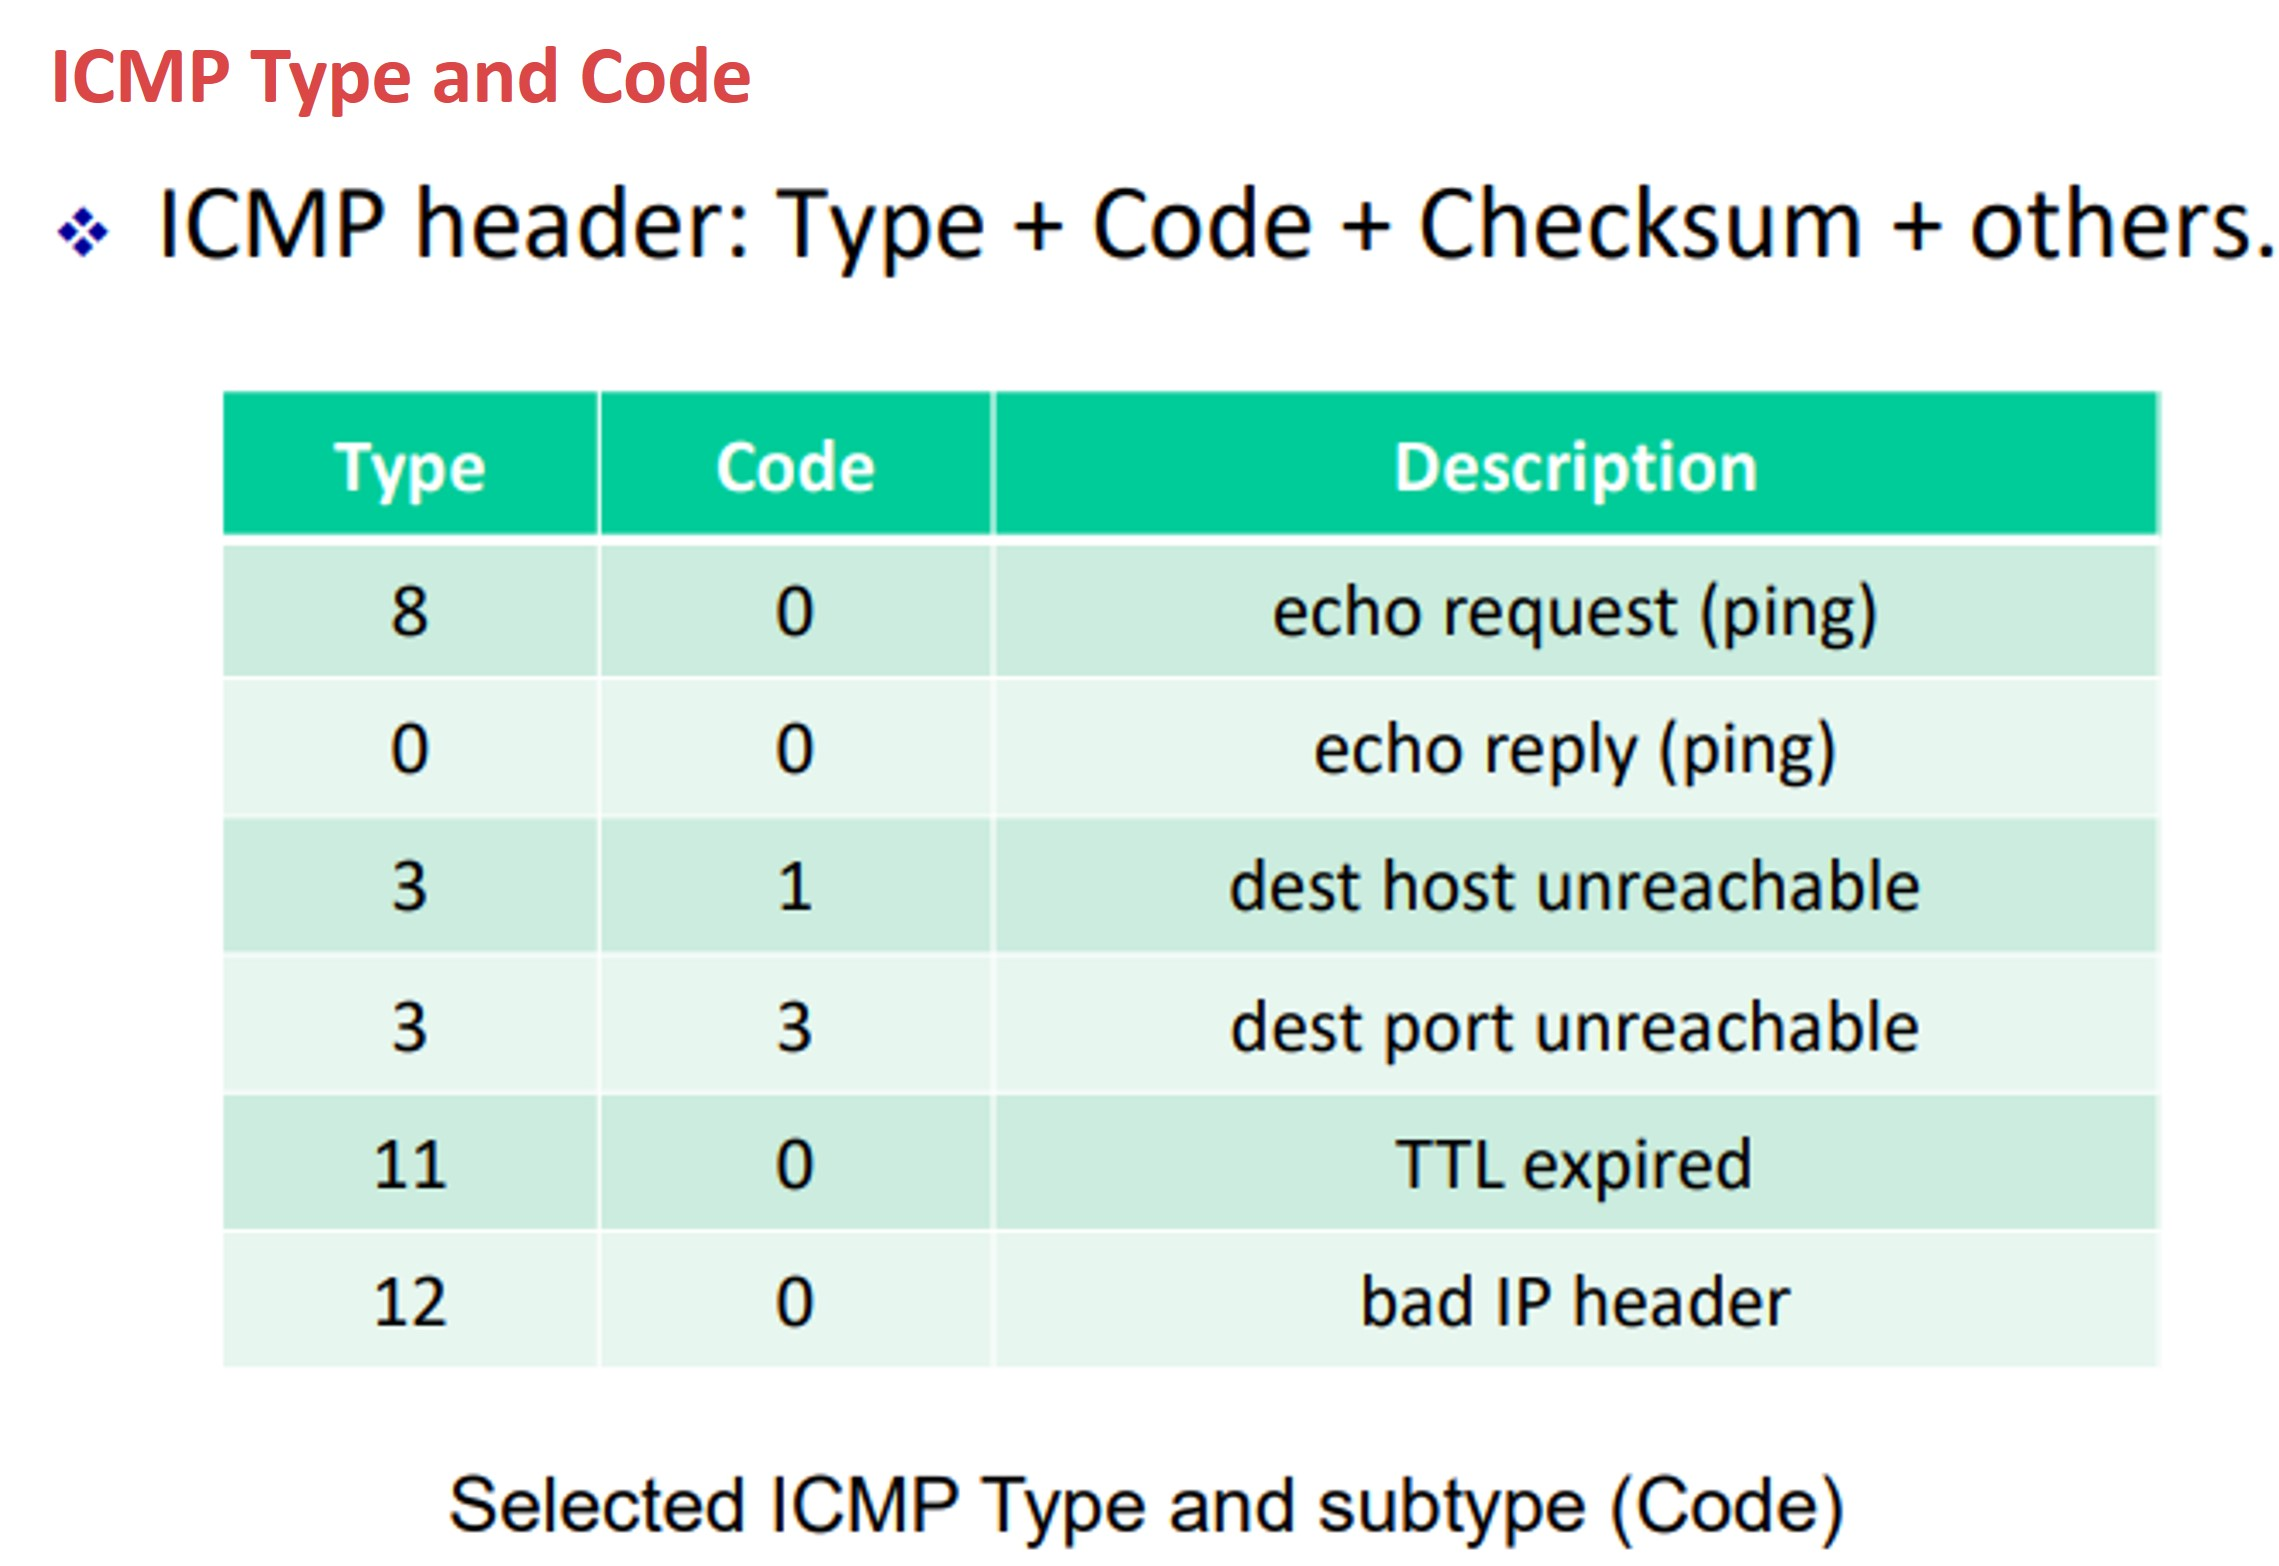
\includegraphics[width=0.7\linewidth]{icmp}}
\end{itemize}











  
  
  
\end{multicols*}
\end{document}